%%%%%%%%%%%%%%%%%%%%%%%%%%%%%%%%%%%%%%%%%%
%Copyright (C) 2018-2020  YuZJLab
%This program is free software: you can redistribute it and/or modify
%it under the terms of the GNU General Public License as published by
%the Free Software Foundation, either version 3 of the License, or
%(at your option) any later version.
%This program is distributed in the hope that it will be useful,
%but WITHOUT ANY WARRANTY; without even the implied warranty of
%MERCHANTABILITY or FITNESS FOR A PARTICULAR PURPOSE.  See the
%GNU General Public License for more details.
%You should have received a copy of the GNU General Public License
%along with this program.  If not, see <https://www.gnu.org/licenses/>.
%%%%%%%%%%%%%%%%%%%%%%%%%%%%%%%%%%%%%%%%%%
\documentclass{book}
\usepackage{xeCJK} %中文支持
\setCJKsansfont{SourceHanSansCN-ExtraLight.otf}
\setCJKmonofont{SourceCodePro-Light.otf}
\setCJKmainfont{SourceHanSerifSC-ExtraLight.otf}
\setCJKfamilyfont{bolded}{SourceHanSansSC-Bold.otf}
\renewcommand{\bf}{\CJKfamily{bolded}}
\newcommand{\normalall}{\normalsize\normalfont\normalcolor}  
\usepackage{color}
\usepackage{graphicx}  %生成图片
\usepackage{geometry} %设置页面排版
\geometry{top=0.5in, bottom=0.5in, left=0.5in, right=0.5in, papersize={21cm,29.7cm}}
\usepackage[super]{nth} %生成序数词
\bibliographystyle{unsrt}
\usepackage{metalogo} %生成TeX标志
\usepackage{texnames} %生成TeX标志
\usepackage{fancybox} %生成带阴影的盒子
\shadowsize=2pt %配置盒子
\usepackage{shorttoc}
\usepackage{flafter}%使得所有浮动体不能被放置在其浮动环境之前
\usepackage{picinpar} %生成文本环绕
\usepackage{indentfirst}%生成段落
\usepackage[toc]{multitoc}%双栏目录
\usepackage{amssymb}%显示方块
\makeatletter\renewcommand{\verbatim@font}{\footnotesize \color{blue}\texttt} \makeatletter%修改verbatim环境格式
 %生成章节中文名和盒子
\renewcommand{\thechapter}{\arabic{chapter}}
\renewcommand{\thesection}{\arabic{chapter}.\arabic{section}}
\renewcommand{\thesubsection}{\arabic{chapter}.\arabic{section}.\arabic{subsection}}
\renewcommand{\thesubsubsection}{\arabic{chapter}.\arabic{section}.\arabic{subsection}.\arabic{subsubsection}}
\usepackage{titlesec}
\renewcommand{\bibname}{参考文献}
\renewcommand{\contentsname}{目录}
\renewcommand{\appendixname}{附录}
\titleformat{\chapter}[frame]{\bf \Huge}{\small 第 \thechapter 部分}{0pt}{}
\titleformat{\section}[frame]{\bf  \LARGE}{\small 第 \thesection 章}{0pt}{}
\titleformat{\subsection}[frame]{\bf  \Large}{\small  第\thesubsection 节}{0pt}{}
\titleformat{\subsubsection}[frame]{\bf \large}{\small 第\thesubsubsection 小节}{0pt}{}
\linespread{1.2} %行距命令
\usepackage{eso-pic}%背景图像命令
\usepackage[backref]{hyperref} %生成书签,这个应被放在末尾
\hypersetup{hidelinks,bookmarks=true,bookmarksopen=true,pdftitle=EMACS 26.2中文手册,pdfauthor=YuZJ}
\begin{document}
\setcounter{tocdepth}{5}
\begin{titlepage}	
\AddToShipoutPictureBG*{\includegraphics[width=21cm,height=29.7cm]{pic/face.png}}
\vspace*{10mm}
\begin{center}
{\color{white}\doublebox{\parbox{18cm}{
\begin{center}	
\Ovalbox{\Huge \bf A GNU Manual:EMACS 26.2中文手册\normalsize}\\\vspace*{5mm}\bf \large 译者:YuZJ \\\vspace*{5mm} 编译日期:\today	
\end{center}}}}
\end{center}
\vspace*{25mm}\normalall
\shadowbox{\parbox[t]{8cm}{{\color{white}{【简介】}}}}
\end{titlepage}
\begin{center}
	\Huge \bf \textbf{$17^{th}$ edition, Updated for Emacs version 26.2}\\中文第1.0版 \normalall
\end{center}
%%%%%%%%%%%%%%%%%%%%%%%%%%%%%%%%%%%%%%%%%%
%Copyright (C) 2018-2020  YuZJLab
%This program is free software: you can redistribute it and/or modify
%it under the terms of the GNU General Public License as published by
%the Free Software Foundation, either version 3 of the License, or
%(at your option) any later version.
%This program is distributed in the hope that it will be useful,
%but WITHOUT ANY WARRANTY; without even the implied warranty of
%MERCHANTABILITY or FITNESS FOR A PARTICULAR PURPOSE.  See the
%GNU General Public License for more details.
%You should have received a copy of the GNU General Public License
%along with this program.  If not, see <https://www.gnu.org/licenses/>.
%%%%%%%%%%%%%%%%%%%%%%%%%%%%%%%%%%%%%%%%%%
\newpage
\vspace*{5cm}
\begin{center}
\Huge GNU Emacs Manual\normalall\\\vspace*{4cm}
Seventeenth Edition, Updated for Emacs Version 26.2.\\\vspace*{5cm}
Richard Stallman et al.
\end{center}
\newpage
\vspace*{8cm}
This is the Seventeenth edition of the GNU Emacs Manual,\par
updated for Emacs version 26.2.\par
Copyright \copyright 1985–1987, 1993–2019 Free Software Foundation, Inc.\par
Permission is granted to copy, distribute and/or modify this document under\par
the terms of the GNU Free Documentation License, Version 1.3 or any later\par
version published by the Free Software Foundation; with the Invariant Sections\par
being “The GNU Manifesto,” “Distribution” and “GNU GENERAL PUBLIC\par
LICENSE,” with the Front-Cover Texts being “A GNU Manual,” and with the\par
Back-Cover Texts as in (a) below. A copy of the license is included in the\par
section entitled “GNU Free Documentation License.”\par
(a) The FSF’s Back-Cover Text is: “You have the freedom to copy and modify\par
this GNU manual. Buying copies from the FSF supports it in developing GNU\par
and promoting software freedom.”\par
Published by the Free Software Foundation\par
51 Franklin Street, Fifth Floor\par
Boston, MA 02110-1301 USA\par
ISBN 978-0-9831592-5-4\par
Cover art by Etienne Suvasa; cover design by Matt Lee.
\shorttoc{简明目录}{1}
\tableofcontents
\chapter{Preface:序言}
This manual documents the use and simple customization of the Emacs editor. Simple Emacs customizations do not  require you to be a programmer, but if you are not interested in customizing, you can ignore the customization hints.\par
这份手册记录了Emacs编辑器的用法和简单的自定义操作。简单的自定义操作不需要你是一个程序员,但如果你对自定义没有兴趣,你可以忽略关于自定义的章节。\par
This is primarily a reference manual, but can also be used as a primer. If you are new to Emacs, we recommend you start with the integrated, learn-by-doing tutorial, before reading the manual. To run the tutorial, start Emacs and type C-h t. The tutorial describes commands, tells you when to try them, and explains the results. The tutorial is available in several languages.\par
这是一份初级的参考手册,但也可以被当成进阶教材使用。如果你对于GNU DEmacs是新手,我们建议你阅读整合的、边做边学的指南。如果你需要查看指南,打开GNU Emacs键入“C-h t\footnote{译注:这个命令的意思是按住Ctrl键的同时按下“h”,再松开这两个键并按下“f”。}”这份指南介绍了常用的命令,告诉你什么时候尝试它们并告诉你结果。这份指南拥有多个语言\footnote{包括简体和繁体中文。请注意如果您使用的是GNU/Linux、BSD或者其他类UNIX操作系统相关发行版的终端模式,中文字符可能无法正确显示。}。\par
On first reading, just skim chapters 1 and 2, which describe the notational conventions of the manual and the general appearance of the Emacs display screen. Note which questions are answered in these chapters, so you can refer back later. After reading chapter 4, you should practice the commands shown there. The next few chapters describe fundamental techniques and concepts that are used constantly. You need to understand them thoroughly, so experiment with them until you are fluent.\par
在你第一次阅读时,请有选择地阅读第一与第二章,这两章介绍了此手册的常规以及Emacs屏幕的常规显示。请注意这两章所回答的问题以便日后查找。在阅读第四章后,请尝试那里的命令。之后几章介绍了最常用的基础的技术和概念。你需要完全理解它们,经常做实验直到十分熟练。\par
Chapters 14 through 19 describe intermediate-level features that are useful for many kinds of editing. Chapter 20 and following chapters describe optional but useful features; read those chapters when you need them.\par
第14到19章介绍了对于多种编辑有用的中间层面的功能。第20章及其以后介绍了可选但是有用的功能;按你所需阅读这些章节。\par
Read the Common Problems chapter if Emacs does not seem to be working properly. It explains how to cope with several common problems (see Section 34.2 [Dealing with Emacs Trouble], page 478), as well as when and how to report Emacs bugs (see Section 34.3 [Bugs], page 482).\par
如果Emacs似乎没有正常工作,阅读“常见问题”章。它解释了如何面对一些常见的问题(参见34.2【处理Emacs问题】),以及何时怎么上报Emacs的问题(参见43.3【问题】)。\par
To find the documentation of a particular command, look in the index. Keys (character commands) and command names have separate indexes. There is also a glossary, with a cross reference for each term.\par
如果你需要查找对于特定命令的支持,参见索引。键(键入命令的字符)与命令名字有不同的索引。还有一个名词索引以查找所有名词。\par
This manual is available as a printed book and also as an Info file. The Info file is for reading from Emacs itself, or with the Info program. Info is the principal format for documentation in the GNU system. The Info file and the printed book contain substantially the same text and are generated from the same source files, which are also distributed with GNU Emacs.\par
这份技术手册同时拥有纸质版和Info文件\footnote{译注:Info是GNU/Linux中的一种帮助系统。}。Info文件可以在Emacs中被阅读或者使用Info程序。Info文件与纸质书由相同的代码生成(同样随GNU Emacs分发)并且包含完全相同的内容。\par
GNU Emacs is a member of the Emacs editor family. There are many Emacs editors, all sharing common principles of organization. For information on the underlying philosophy of Emacs and the lessons learned from its development, see \textit{Emacs, the Extensible, Customizable Self-Documenting Display Editor}, available from \url{http://hdl.handle.net/1721.1/5736}.\par
GNU Emacs是Emacs编辑器家族的一员。目前有许多Emacs编辑器,它们共用相同的组织准则。对于有关Emacs现行的哲学以及从Emacs发展中得到的教训,参见\url{http://hdl.handle.net/1721.1/5736}的文章《Emacs, the Extensible, Customizable Self-Documenting Display Editor》。\par
This version of the manual is mainly intended for use with GNU Emacs installed on GNU and Unix systems. GNU Emacs can also be used on MS-DOS, Microsoft Windows, and Macintosh systems. The Info file version of this manual contains some more information about using Emacs on those systems. Those systems use different file name syntax; in addition MS-DOS does not support all GNU Emacs features. See Appendix G [Microsoft Windows], page 542, for information about using Emacs on Windows. See Appendix F [Mac OS / GNUstep], page 539, for information about using Emacs on Macintosh (and
GNUstep).\par
这个版本的手册主要是为了安装在GNU与UNIX操作系统上的GNU Emacs设计的,GNU Emacs也在MS-DOS、微软视窗操作系统与麦金塔机上使用。这份手册的Info文件版本包括这些系统上的更多信息。这些操作系统使用不同的文件名;并且MS-DOS也不完全支持GNU Emacs的功能。参见附录【微软视窗操作系统】以查找视窗操作系统上使用的GNU Emacs的相关信息。参见附录【MacOS/GNUstep】以查找在麦金塔机上使用GNU Emacs的信息。
\chapter{Distribution:分发}
GNU Emacs is free software; this means that everyone is free to use it and free to redistribute it under certain conditions. GNU Emacs is not in the public domain; it is copyrighted and there are restrictions on its distribution, but these restrictions are designed to permit everything that a good cooperating citizen would want to do. What is not allowed is to try to prevent others from further sharing any version of GNU Emacs that they might get from you. The precise conditions are found in the GNU General Public License that comes with Emacs and also appears in this manual\footnote{This manual is itself covered by the GNU Free Documentation License. This license is similar in spirit to the General Public License, but is more suitable for documentation. See Appendix B [GNU Free Documentation License]}. See Appendix A [Copying], page 495.\par
GNU Emacs 是自由软件;这意味着所有人都能在不违反相关条例的情况下自由地使用和重新构建。GNU Emacs并不被放在公共区域\footnote{译注:也就是说,你不能为所欲为。};它是受到版权保护并且其分发是有限制的。但是这些限制的目的是保证一个品行端正且愿意合作的公民做其所希望做的事情的自由。试图防止他人分享可能从你那里得到的任何GNU Emacs版本是被禁止的。精确的条例将可以在随附GNU Emacs提供的GNU General Public Licence或者这份手册\footnote{这份手册本身是受GNU Free Documentation License保护的:它的精神接近GNU General Public License,但更适合用于文档。参见附录【GNU Free Documentation License】}的底部:参见附录【GNU General Public License】,第\pageref{chap:gpl}页。\par
One way to get a copy of GNU Emacs is from someone else who has it. You need not ask for our permission to do so, or tell anyone else; just copy it. If you have access to the Internet, you can get the latest distribution version of GNU Emacs by anonymous FTP; see \url{https://www.gnu.org/software/emacs} on our website for more information.\par
一种得到GNU Emacs副本的方法是从其他拥有副本的人那里获取。你不需要为此事征求许可或告诉任何其他人;你只需要复制它即可。如果你能连接到互联网,你可以从匿名的FTP服务器\footnote{译注:FTP是“文件共享协议”的缩写,你能够从搭建FTP服务器的站点下载文件。}中得到GNU Emacs的最新副本;参见\url{https://www.gnu.org/software/emacs}以得到更多信息。\par
You may also receive GNU Emacs when you buy a computer. Computer manufacturers are free to distribute copies on the same terms that apply to everyone else. These terms require them to give you the full sources, including whatever changes they may have made, and to permit you to redistribute the GNU Emacs received from them under the usual terms of the General Public License. In other words, the program must be free for you when you get it, not just free for the manufacturer.\par
你也可能在你购买电脑时获得一份GNU Emacs副本\footnote{译注:从目前的主流制造商来看,这似乎不太可能。}。计算机制造商可以按照适用于其他人的条例自由地分发GNU Emacs。这些条款要求他们给出包含他们所做出的改变的完整的源代码,并且允许你按照GNU General Public License重建从他们那里获得的GNU Emacs。换言之,这个程序必须在你获得它是是自由的,而不是仅对生产商自由。\par
If you find GNU Emacs useful, please send a donation to the Free Software Foundation to support our work. Donations to the Free Software Foundation are tax-deductible in the US. If you use GNU Emacs at your workplace, please suggest that the company make a donation. To donate, see \url{https://my.fsf.org/donate/}. For other ways in which you can help, see \url{https://www.gnu.org/help/help.html}.\par
如果你觉得GNU Emacs有用,请捐款给自由软件基金会(Free Software Foundation)以支持我们。对于自由软件基金会的捐赠在美国是免税的。如果你在你的工作处使用GNU Emacs,请建议你的公司作出捐赠。如果你对于捐赠感兴趣,请看\url{https://my.fsf.org/donate/}。你也可以参照\url{https://www.gnu.org/help/help.html}如果你希望以其他形式提供帮助。\par
We also sell hardcopy versions of this manual and \textit{An Introduction to Programming in Emacs Lisp}, by Robert J. Chassell. You can visit our online store at \url{https://shop.fsf.org/}. The income from sales goes to support the foundation’s purpose: the development of new free software, and improvements to our existing programs including GNU Emacs.\par
我们也出售这份手册的纸质版本\footnote{译注:当然,这里指的是没有中文翻译的原版。}以及由Robert J. Chassell编著的《An Introduction to Programming in Emacs Lisp》。你可以在\url{https://shop.fsf.org/}浏览我们的在线商店,它的收入被用于支持基金会的意图:新软件的开发以及旧软件(包括GNU Emacs)的提高。\par
If you need to contact the Free Software Foundation, see\url{ https://www.fsf.org/about/contact/}, or write to\par
如果你希望与自由软件基金会联系,参见\url{ https://www.fsf.org/about/contact/}或者写信给:\par
Free Software Foundation\par
51 Franklin Street, Fifth Floor\par
Boston, MA 02110-1301\par
USA
\section{英文版致谢}
Contributors to GNU Emacs include (为GNU Emacs提供贡献的包括) Jari Aalto, Per Abrahamsen, Tomas Abrahamsson, Jay K. Adams, Alon Albert, Michael Albinus, Nagy Andras, Benjamin Andresen, Ralf Angeli, Dmitry Antipov, Joe Arceneaux, Emil ˚ Astr¨om, Miles Bader, David Bakhash, Juanma Barranquero, Eli Barzilay, Thomas Baumann, Steven L. Baur, Jay Belanger, Alexander L. Belikoff, Thomas Bellman, Scott Bender, Boaz Ben-Zvi, Sergey Berezin, Stephen Berman, Karl Berry, Anna M. Bigatti, Ray Blaak, Martin Blais, Jim Blandy, Johan Bockg˚ard, Jan B¨ocker, Joel Boehland, Lennart Borgman, Per Bothner, Terrence Brannon, Frank Bresz, Peter Breton, Emmanuel Briot, Kevin Broadey, Vincent Broman, Michael Brouwer, David M. Brown, Ken Brown, Stefan Bruda, Georges Brun-Cottan, Joe Buehler, Scott Byer, W lodek Bzyl, Tino Calancha, Bill Carpenter, Per Cederqvist, Hans Chalupsky, Chris Chase, Bob Chassell, Andrew Choi, Chong Yidong, Sacha Chua, Stewart Clamen, James Clark, Mike Clarkson, Glynn Clements, Andrew Cohen, Daniel Colascione, Christoph Conrad, Ludovic Court`es, Andrew Csillag, Toby Cubitt, Baoqiu Cui, Doug Cutting, Mathias Dahl, Julien Danjou, Satyaki Das, Vivek Dasmohapatra, Dan Davison, Michael DeCorte, Gary Delp, Nachum Dershowitz, Dave Detlefs, Matthieu Devin, Christophe de Dinechin, Eri Ding, Jan Dj¨arv, Lawrence R. Dodd, Carsten Dominik, Scott Draves, Benjamin Drieu, Viktor Dukhovni, Jacques Duthen, Dmitry Dzhus, John Eaton, Rolf Ebert, Carl Edman, David Edmondson, Paul Eggert, Stephen Eglen, Christian Egli, Torbj¨orn Einarsson, Tsugutomo Enami, David Engster, Hans Henrik Eriksen, Michael Ernst, Ata Etemadi, Frederick Farnbach, Oscar Figueiredo, Fred Fish, Steve Fisk, Karl Fogel, Gary Foster, Eric S. Fraga, Romain Francoise, Noah Friedman, Andreas Fuchs, Shigeru Fukaya, Xue Fuqiao, Hallvard Furuseth, Keith Gabryelski, Peter S. Galbraith, Kevin Gallagher, Fabi´an E. Gallina, Kevin Gallo, Juan Le´on Lahoz Garc´ıa, Howard Gayle, Daniel German, Stephen Gildea, Julien Gilles, David Gillespie, Bob Glickstein, Deepak Goel, David De La Harpe Golden, Boris Goldowsky, David Goodger, Chris Gray, Kevin Greiner, Michelangelo Grigni, Odd Gripenstam, Kai Großjohann, Michael Gschwind, Bastien Guerry, Henry Guillaume, Dmitry Gutov, Doug Gwyn, Bruno Haible, Ken’ichi Handa, Lars Hansen, Chris Hanson, Jesper Harder, Alexandru Harsanyi, K. Shane Hartman, John Heidemann, Jon K. Hellan, Magnus Henoch, Markus Heritsch, Dirk Herrmann, Karl Heuer, Manabu Higashida, Konrad Hinsen, Anders Holst, Jeffrey C. Honig, Tassilo Horn, Kurt Hornik, Tom Houlder, Joakim Hove, Denis Howe, Lars Ingebrigtsen, Andrew Innes, Seiichiro Inoue, Philip Jackson, Martyn Jago, Pavel Janik, Paul Jarc, Ulf Jasper, Thorsten Jolitz, Michael K. Johnson, Kyle Jones, Terry Jones, Simon Josefsson, Alexandre Julliard, Arne Jørgensen, Tomoji Kagatani, Brewster Kahle, Tokuya Kameshima, Lute Kamstra, Ivan Kanis, David Kastrup, David Kaufman, Henry Kautz, Taichi Kawabata, Taro Kawagishi, Howard Kaye, Michael Kifer, Richard King, Peter Kleiweg, Karel Kl´ıˇc, Shuhei Kobayashi, Pavel Kobyakov, Larry K. Kolodney, David M. Koppelman, Koseki Yoshinori, Robert Krawitz, Sebastian Kremer, Ryszard Kubiak, Igor Kuzmin, David K˚agedal, Daniel LaLiberte, Karl Landstrom, Mario Lang, Aaron Larson, James R. Larus, Vinicius Jose Latorre, Werner Lemberg, Frederic Lepied, Peter Liljenberg, Christian Limpach, Lars Lindberg, Chris Lindblad, Anders Lindgren, Thomas Link, Juri Linkov, Francis Litterio, Sergey Litvinov, Leo Liu, Emilio C. Lopes, Martin Lorentzon, Dave Love, Eric Ludlam, K´aroly L˝orentey, Sascha L¨udecke, Greg McGary, Roland McGrath, Michael McNamara, Alan Mackenzie, Christopher J. Madsen, Neil M. Mager, Artur Malabarba, Ken Manheimer, Bill Mann, Brian Marick, Simon Marshall, Bengt Martensson, Charlie Martin, Yukihiro Matsumoto, Tomohiro Matsuyama, David Maus, Thomas May, Will Mengarini, David Megginson, Stefan Merten, Ben A. Mesander, Wayne Mesard, Brad Miller, Lawrence Mitchell, Richard Mlynarik, Gerd M¨ollmann, Dani Moncayo, Stefan Monnier, Keith Moore, Jan Moringen, Morioka Tomohiko, Glenn Morris, Don Morrison, Diane Murray, Riccardo Murri, Sen Nagata, Erik Naggum, Gergely Nagy, Nobuyoshi Nakada, Thomas Neumann, Mike Newton, Thien-Thi Nguyen, Jurgen Nickelsen, Dan Nicolaescu, Hrvoje Nikˇsi´c, Jeff Norden, Andrew Norman, Theresa O’Connor, Kentaro Ohkouchi, Christian Ohler, Kenichi Okada, Alexandre Oliva, Bob Olson, Michael Olson, Takaaki Ota, Mark Oteiza, Pieter E. J. Pareit, Ross Patterson, David Pearson, Juan Pechiar, Jeff Peck, Damon Anton Permezel, Tom Perrine, William M. Perry, Per Persson, Jens Petersen, Nicolas Petton, Daniel Pfeiffer, Justus Piater, Richard L. Pieri, Fred Pierresteguy, Fran¸cois Pinard, Daniel Pittman, Christian Plaunt, Alexander Pohoyda, David Ponce, Noam Postavsky, Francesco A. Potort`ı, Michael D. Prange, Mukesh Prasad, Ken Raeburn, Marko Rahamaa, Ashwin Ram, Eric S. Raymond, Paul Reilly, Edward M. Reingold, David Reitter, Alex Rezinsky, Rob Riepel, Lara Rios, Adrian Robert, Nick Roberts, Roland B. Roberts, John Robinson, Denis B. Roegel, Danny Roozendaal, Sebastian Rose, William Rosenblatt, Markus Rost, Guillermo J. Rozas, Martin Rudalics, Ivar Rummelhoff, Jason Rumney, Wolfgang Rupprecht, Benjamin Rutt, Kevin Ryde, James B. Salem, Masahiko Sato, Timo Savola, Jorgen Sch¨afer, Holger Schauer, William Schelter, Ralph Schleicher, Gregor Schmid, Michael Schmidt, Ronald S. Schnell, Philippe Schnoebelen, Jan Schormann, Alex Schroeder, Stefan Schoef, Rainer Sch¨opf, Raymond Scholz, Eric Schulte, Andreas Schwab, Randal Schwartz, Oliver Seidel, Manuel Serrano, Paul Sexton, Hovav Shacham, Stanislav Shalunov, Marc Shapiro, Richard Sharman, Olin Shivers, Tibor Simko, Espen Skoglund, Rick Sladkey, Lynn Slater, Chris Smith, David ˇ Smith, Paul D. Smith, Wilson Snyder, William Sommerfeld, Simon South, Andre Spiegel, Michael Staats, Thomas Steffen, Ulf Stegemann, Reiner Steib, Sam Steingold, Ake Stenhoff, Philipp Stephani, Peter Stephenson, Ken Stevens, Andy Stewart, Jonathan Stigelman, Martin Stjernholm, Kim F. Storm, Steve Strassmann, Christopher Suckling, Olaf Sylvester, Naoto Takahashi, Steven Tamm, Jan Tatarik, Luc Teirlinck, Jean-Philippe Theberge, Jens T. Berger Thielemann, Spencer Thomas, Jim Thompson, Toru Tomabechi, David O’Toole, Markus Triska, Tom Tromey, Enami Tsugutomo, Eli Tziperman, Daiki Ueno, Masanobu Umeda, Rajesh Vaidheeswarran, Neil W. Van Dyke, Didier Verna, Joakim Verona, Ulrik Vieth, Geoffrey Voelker, Johan Vromans, Inge Wallin, John Paul Wallington, Colin Walters, Barry Warsaw, Christoph Wedler, Ilja Weis, Zhang Weize, Morten Welinder, Joseph Brian Wells, Rodney Whitby, John Wiegley, Sascha Wilde, Ed Wilkinson, Mike Williams, Roland Winkler, Bill Wohler, Steven A. Wood, Dale R. Worley, Francis J. Wright, Felix S. T. Wu, Tom Wurgler, Yamamoto Mitsuharu, Katsumi Yamaoka, Masatake Yamato, Jonathan Yavner, Ryan Yeske, Ilya Zakharevich, Milan Zamazal, Victor Zandy, Eli Zaretskii, Jamie Zawinski, Andrew Zhilin, Shenghuo Zhu, Piotr Zieli´nski, Ian T. Zimmermann, Reto Zimmermann, Neal Ziring, Teodor Zlatanov, and Detlev Zundel.
\chapter{Introduction:对于GNU Emacs的介绍}
You are reading about GNU Emacs, the GNU incarnation of the advanced, self-documenting, customizable, extensible editor Emacs. (The ‘G’ in GNU (GNU’s Not Unix) is not silent.)\par
你正在阅读GNU Emacs,高级的、具有完全帮助的、可完全自定义的、可扩展的编辑器Emacs的GNU版本(GNU(GNU's Not Unix)中的“G”不是不发音的)。\par
We call Emacs \textit{advanced} because it can do much more than simple insertion and deletion of text. It can control subprocesses, indent programs automatically, show multiple files at once, and more. Emacs editing commands operate in terms of characters, words, lines, sentences, paragraphs, and pages, as well as expressions and comments in various programming languages.\par
我们称Emacs“高级的”因为它能够做除了简单的插入和删除以外的很多事。它能够控制子进程,同时展示多个文件等等。Emacs的编辑命令是靠键入字符、单词、句子、段落和页面以及各种编程语言的表达和注释完成的。\par
\textit{Self-documenting} means that at any time you can use special commands, known as help commands, to find out what your options are, or to find out what any command does, or to find all the commands that pertain to a given topic. See Chapter 7 [Help], page 39.\par
“具有完全帮助的”意为任何时候你可以使用称为“帮助命令”的特殊命令来明白你的操作是什么,或者其它命令将会干什么,或者找到关于特定主体的所有命令。参见第七章【帮助】。\par
\textit{Customizable} means that you can easily alter the behavior of Emacs commands in simple ways. For instance, if you use a programming language in which comments start with ‘<**’ and end with ‘**>’, you can tell the Emacs comment manipulation commands to use those strings (see Section 23.5 [Comments], page 268). To take another example, you can rebind the basic cursor motion commands (up, down, left and right) to any keys on the keyboard that you find comfortable. See Chapter 33 [Customization], page 444.\par
“可完全自定义的”意为你能够易如反掌地改变Emacs命令的用法。比如说,如果你使用一种注释由“<**”开头,由“**>”结尾的编程语言,你可以告诉Emacs的注释操作命令使用这些字符串(参见23.5节【注释】)。再举个例子:你可以将基本光标移动命令(上、下、左、右)重新关联到你觉得舒服的不同键。参见第33章【自定义】。\par
\textit{Extensible} means that you can go beyond simple customization and create entirely new commands. New commands are simply programs written in the Lisp language, which are run by Emacs’s own Lisp interpreter. Existing commands can even be redefined in the middle of an editing session, without having to restart Emacs. Most of the editing commands in Emacs are written in Lisp; the few exceptions could have been written in Lisp but use C instead for efficiency. Writing an extension is programming, but non-programmers can use it afterwards. See Section “Preface” in \textit{An Introduction to Programming in Emacs Lisp}, if you want to learn Emacs Lisp programming.\par
“可扩展的”意为你能够越过简单的自定义创建自己的新命令。新命令应是由Lisp语言书写的,由Emacs自己的Lisp解释器执行的程序。甚至连“退出”指令都能够在编辑时被重新定义。大多数编辑命令都是有Lisp书写的;特殊的排除项虽然也能够使用Lisp书写,但为了更强大的效率使用C语言。写扩展是编程,但是非编程人员可以在之后使用它。如果你想要学习Lisp编程,请参见《An Introduction to Programming in Emacs Lisp》的“Preface”章节。
%%%%%%%%%%%%%%%%%%%%%%%%%%%%%%%%%%%%%%%%%%
%Copyright (C) 2018-2020  YuZJLab
%This program is free software: you can redistribute it and/or modify
%it under the terms of the GNU General Public License as published by
%the Free Software Foundation, either version 3 of the License, or
%(at your option) any later version.
%This program is distributed in the hope that it will be useful,
%but WITHOUT ANY WARRANTY; without even the implied warranty of
%MERCHANTABILITY or FITNESS FOR A PARTICULAR PURPOSE.  See the
%GNU General Public License for more details.
%You should have received a copy of the GNU General Public License
%along with this program.  If not, see <https://www.gnu.org/licenses/>.
%%%%%%%%%%%%%%%%%%%%%%%%%%%%%%%%%%%%%%%%%%
\chapter{The Organization of the Screen:屏幕的组织结构}
On a graphical display, such as on GNU/Linux using the X Window System, Emacs occupies
a graphical window. On a text terminal, Emacs occupies the entire terminal screen. We
will use the term frame to mean a graphical window or terminal screen occupied by Emacs.
Emacs behaves very similarly on both kinds of frames. It normally starts out with just one
frame, but you can create additional frames if you wish (see Chapter 18 [Frames]).
\par
在一个图形界面(例如,使用X Windows系统的GNU/Linux操作系统)中,Emacs占用了一个图形窗口(Window)。在一个文本终端中,Emacs占用了一整个终端屏幕。我们将会使用“窗体”(Frame)表示Emacs占用的图形窗体或终端屏幕。Emacs在这两种窗体下表现十分相似\footnote{译注:虽然我不这么认为}。一般情况下Emacs在启动时创建一个窗体,但是你可以按照你的意愿创建另外的窗体(参见第18章【窗体】)。\par
Each frame consists of several distinct regions. At the top of the frame is a menu bar,
which allows you to access commands via a series of menus. On a graphical display, directly
below the menu bar is a tool bar, a row of icons that perform editing commands when you
click on them. At the very bottom of the frame is an echo area, where informative messages
are displayed and where you enter information when Emacs asks for it.
\par
Emacs窗体包括多个区分明显的区域。在窗体的最顶端是菜单栏(Menu Bar),它允许你通过一系列菜单访问命令。在一个图形界面上,菜单栏下方是工具栏(Tool Bar)。它由一系列图标构成,当你单击它是它将执行编辑命令。回显区(Echo Area)窗体的最底端,用于显示Emacs的提示信息或者当Emacs需要你输入时键入信息。\par
The main area of the frame, below the tool bar (if one exists) and above the echo area, is
called the window. Henceforth in this manual, we will use the word “window” in this sense.
Graphical display systems commonly use the word “window” with a different meaning; but,
as stated above, we refer to those graphical windows as “frames”.
\par
在一个Emacs窗体中,位于工具栏(如果存在的话)以及回显区的大块区域称为窗格(Window)。此后我们将会使用“窗格”来表示这个意思。图形界面系统一般会使用“窗口”(Window)来表示不同的意思;但是,正如已经声明的一样,我们将称这些图形界面窗口为“窗体”(Frame)。\par
An Emacs window is where the buffer—the text or other graphics you are editing or
viewing—is displayed. On a graphical display, the window possesses a scroll bar on one
side, which can be used to scroll through the buffer. The last line of the window is a mode
line. This displays various information about what is going on in the buffer, such as whether
there are unsaved changes, the editing modes that are in use, the current line number, and
so forth.
\par
缓冲区(Buffer)——文本、图像以及其他你正在编辑或浏览的东西所显示的地方——位于Emacs窗口。在一个图形界面上,窗格\footnote{译注:是“Window”。此后窗格一律称“Window”,窗体一律称“Frame”。窗口?那是什么东西?}拥有一个纵向的滚动条用于滚动显示整个缓冲区。窗格的最底端一栏(在终端界面下是一行文字)称为状态栏(Mode Line),用于显示关于缓冲区中正在进行的操作的的信息,比如说是否有未保存的改变,正在使用的编辑模式(Editing Mode),当前的行号等等。\par
When you start Emacs, there is normally only one window in the frame. However, you
can subdivide this window horizontally or vertically to create multiple windows, each of
which can independently display a buffer (see Chapter 17 [Windows]).
\par
通常情况下,当你启动Emacs的时候,一个窗体中只有一个窗格。但是,你可以将这个窗格水平或竖直地分为多个窗格,它们各自独立地显示一个缓冲区(参见第17章【窗格】)。\par
At any time, one window is the selected window. On a graphical display, the selected
window shows a more prominent cursor (usually solid and blinking); other windows show a
less prominent cursor (usually a hollow box). On a text terminal, there is only one cursor,
which is shown in the selected window. The buffer displayed in the selected window is
called the current buffer, and it is where editing happens. Most Emacs commands implicitly
apply to the current buffer; the text displayed in unselected windows is mostly visible for
reference. If you use multiple frames on a graphical display, selecting a particular frame
selects a window in that frame.\par
在任何时候,有且仅有一个窗格是活动窗格(Selected Window)。在一个图形界面下,活动窗格显示一个更加明显的光标(Crusor)(一般是闪动的黑色方块“$\blacksquare$”);其它窗格显示一个不明显的光标(一般是空心方块“$\square$”)。终端界面只将在活动窗格显示一个光标。在活动窗格显示的缓冲区称为活动缓冲区(“Selected Buffer”)并且就是正在被编辑的缓冲区。大部分Emacs命令含蓄地作用于活动缓冲区;在非活动的缓冲区中显示的文字仅仅为参考而显示。如果你使用多窗体的图形界面,选择一个窗体再选择一个窗格。
\begin{center}
	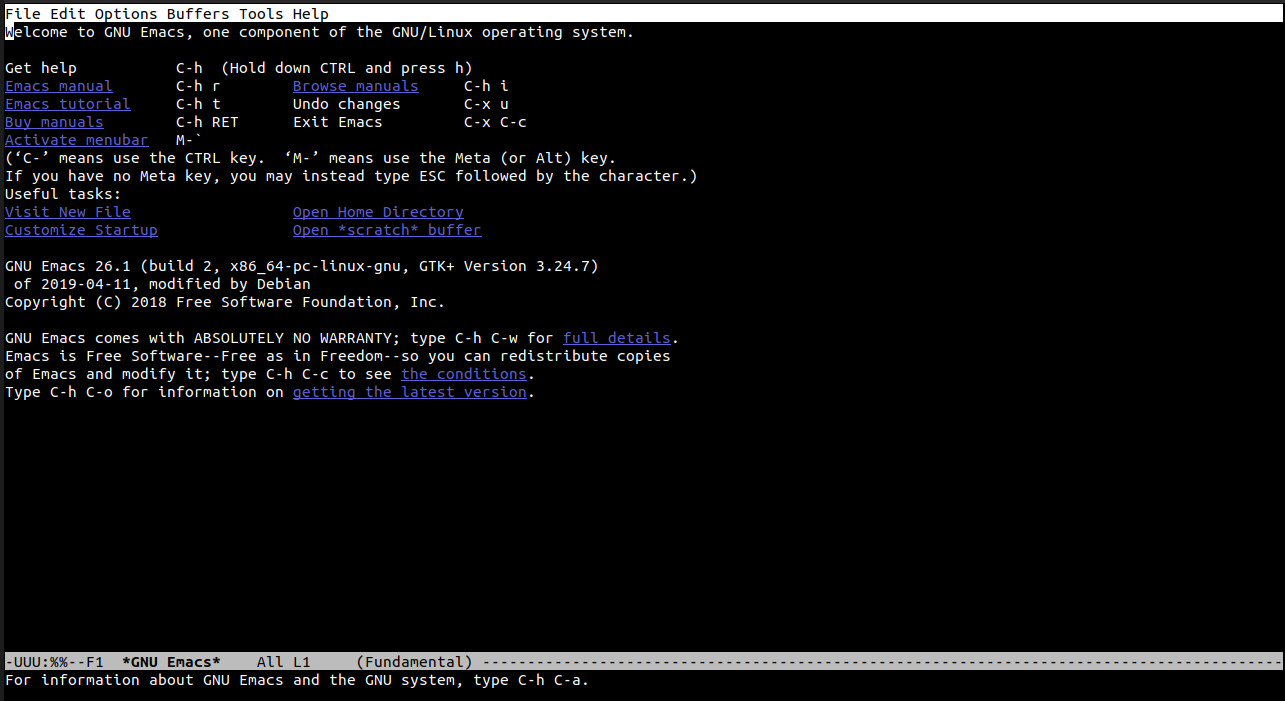
\includegraphics[scale=0.4]{pic/Emacs-Terminal-Defaut}
\end{center}
\section{Point:点}
The cursor in the selected window shows the location where most editing commands take effect, which is called point\footnote{The term “point” comes from the character ‘.’, which was the command in TECO (the language in which the original Emacs was written) for accessing the editing position.}. Many Emacs commands move point to different places in the buffer; for example, you can place point by clicking mouse button 1 (normally the left button) at the desired location.\par
位于被选中窗口的光标(称作“点”,point\footnote{“点”来自于字符“.”,是TECO语言(最初的Emacs由该语言写成)用于连接到正在编辑的位置的命令。})显示了大多数编辑命令生效的位置。许多Emacs的命令能够在缓冲区之内移动光标
\appendix
%%%%%%%%%%%%%%%%%%%%%%%%%%%%%%%%%%%%%%%%%%
%Copyright (C) 2018-2020  YuZJLab
%This program is free software: you can redistribute it and/or modify
%it under the terms of the GNU General Public License as published by
%the Free Software Foundation, either version 3 of the License, or
%(at your option) any later version.
%This program is distributed in the hope that it will be useful,
%but WITHOUT ANY WARRANTY; without even the implied warranty of
%MERCHANTABILITY or FITNESS FOR A PARTICULAR PURPOSE.  See the
%GNU General Public License for more details.
%You should have received a copy of the GNU General Public License
%along with this program.  If not, see <https://www.gnu.org/licenses/>.
%%%%%%%%%%%%%%%%%%%%%%%%%%%%%%%%%%%%%%%%%%
\chapter{GNU GENERAL PUBLIC LICENSE}
\begin{center} Version 3, 29 June 2007 \end{center}
Copyright \copyright 2007 Free Software Foundation, Inc. <\url{https://fsf.org/}>\par
Everyone is permitted to copy and distribute verbatim copies of this license document, but changing it is not allowed.\par
\section{Preamble}
The GNU General Public License is a free, copyleft license for software and other kinds of works.\par
The licenses for most software and other practical works are designed to take away your freedom to share and change the works. By contrast, the GNU General Public License is intended to guarantee your freedom to share and change all versions of a program--to make sure it remains free software for all its users. We, the Free Software Foundation, use the GNU General Public License for most of our software; it applies also to any other work released this way by its authors. You can apply it to your programs, too.\par
When we speak of free software, we are referring to freedom, not price. Our General Public Licenses are designed to make sure that you have the freedom to distribute copies of free software (and charge for them if you wish), that you receive source code or can get it if you want it, that you can change the software or use pieces of it in new free programs, and that you know you can do these things.\par
To protect your rights, we need to prevent others from denying you these rights or asking you to surrender the rights. Therefore, you have certain responsibilities if you distribute copies of the software, or if you modify it: responsibilities to respect the freedom of others.\par
For example, if you distribute copies of such a program, whether gratis or for a fee, you must pass on to the recipients the same freedoms that you received. You must make sure that they, too, receive or can get the source code. And you must show them these terms so they know their rights.\par
Developers that use the GNU GPL protect your rights with two steps: (1) assert copyright on the software, and (2) offer you this License giving you legal permission to copy, distribute and/or modify it.\par
For the developers' and authors' protection, the GPL clearly explains that there is no warranty for this free software. For both users' and authors' sake, the GPL requires that modified versions be marked as changed, so that their problems will not be attributed erroneously to authors of previous versions.\par
Some devices are designed to deny users access to install or run modified versions of the software inside them, although the manufacturer can do so. This is fundamentally incompatible with the aim of protecting users' freedom to change the software. The systematic pattern of such abuse occurs in the area of products for individuals to use, which is precisely where it is most unacceptable. Therefore, we have designed this version of the GPL to prohibit the practice for those products. If such problems arise substantially in other domains, we stand ready to extend this provision to those domains in future versions of the GPL, as needed to protect the freedom of users.\par
Finally, every program is threatened constantly by software patents. States should not allow patents to restrict development and use of software on general-purpose computers, but in those that do, we wish to avoid the special danger that patents applied to a free program could make it effectively proprietary. To prevent this, the GPL assures that patents cannot be used to render the program non-free.\par
The precise terms and conditions for copying, distribution and modification follow.
\section{TERMS AND CONDITIONS}
\subsubsection{0. Definitions.}
“This License” refers to version 3 of the GNU General Public License.\par
“Copyright” also means copyright-like laws that apply to other kinds of works, such as semiconductor masks.\par
“The Program” refers to any copyrightable work licensed under this License. Each licensee is addressed as “you”. “Licensees” and “recipients” may be individuals or organizations.\par
To “modify” a work means to copy from or adapt all or part of the work in a fashion requiring copyright permission, other than the making of an exact copy. The resulting work is called a “modified version” of the earlier work or a work “based on” the earlier work.\par
A “covered work” means either the unmodified Program or a work based on the Program.\par
To “propagate” a work means to do anything with it that, without permission, would make you directly or secondarily liable for infringement under applicable copyright law, except executing it on a computer or modifying a private copy. Propagation includes copying, distribution (with or without modification), making available to the public, and in some countries other activities as well.\par
To “convey” a work means any kind of propagation that enables other parties to make or receive copies. Mere interaction with a user through a computer network, with no transfer of a copy, is not conveying.\par
An interactive user interface displays “Appropriate Legal Notices” to the extent that it includes a convenient and prominently visible feature that (1) displays an appropriate copyright notice, and (2) tells the user that there is no warranty for the work (except to the extent that warranties are provided), that licensees may convey the work under this License, and how to view a copy of this License. If the interface presents a list of user commands or options, such as a menu, a prominent item in the list meets this criterion.
\subsubsection{1. Source Code.}
The “source code” for a work means the preferred form of the work for making modifications to it. “Object code” means any non-source form of a work.\par
A “Standard Interface” means an interface that either is an official standard defined by a recognized standards body, or, in the case of interfaces specified for a particular programming language, one that is widely used among developers working in that language.\par
The “System Libraries” of an executable work include anything, other than the work as a whole, that (a) is included in the normal form of packaging a Major Component, but which is not part of that Major Component, and (b) serves only to enable use of the work with that Major Component, or to implement a Standard Interface for which an implementation is available to the public in source code form. A “Major Component”, in this context, means a major essential component (kernel, window system, and so on) of the specific operating system (if any) on which the executable work runs, or a compiler used to produce the work, or an object code interpreter used to run it.\par
The “Corresponding Source” for a work in object code form means all the source code needed to generate, install, and (for an executable work) run the object code and to modify the work, including scripts to control those activities. However, it does not include the work's System Libraries, or general-purpose tools or generally available free programs which are used unmodified in performing those activities but which are not part of the work. For example, Corresponding Source includes interface definition files associated with source files for the work, and the source code for shared libraries and dynamically linked subprograms that the work is specifically designed to require, such as by intimate data communication or control flow between those subprograms and other parts of the work.\par
The Corresponding Source need not include anything that users can regenerate automatically from other parts of the Corresponding Source.\par
The Corresponding Source for a work in source code form is that same work.
\subsubsection{2. Basic Permissions.}
All rights granted under this License are granted for the term of copyright on the Program, and are irrevocable provided the stated conditions are met. This License explicitly affirms your unlimited permission to run the unmodified Program. The output from running a covered work is covered by this License only if the output, given its content, constitutes a covered work. This License acknowledges your rights of fair use or other equivalent, as provided by copyright law.\par
You may make, run and propagate covered works that you do not convey, without conditions so long as your license otherwise remains in force. You may convey covered works to others for the sole purpose of having them make modifications exclusively for you, or provide you with facilities for running those works, provided that you comply with the terms of this License in conveying all material for which you do not control copyright. Those thus making or running the covered works for you must do so exclusively on your behalf, under your direction and control, on terms that prohibit them from making any copies of your copyrighted material outside their relationship with you.\par
Conveying under any other circumstances is permitted solely under the conditions stated below. Sublicensing is not allowed; section 10 makes it unnecessary.
\subsubsection{3. Protecting Users' Legal Rights From Anti-Circumvention Law.}
No covered work shall be deemed part of an effective technological measure under any applicable law fulfilling obligations under article 11 of the WIPO copyright treaty adopted on 20 December 1996, or similar laws prohibiting or restricting circumvention of such measures.\par
When you convey a covered work, you waive any legal power to forbid circumvention of technological measures to the extent such circumvention is effected by exercising rights under this License with respect to the covered work, and you disclaim any intention to limit operation or modification of the work as a means of enforcing, against the work's users, your or third parties' legal rights to forbid circumvention of technological measures.
\subsubsection{4. Conveying Verbatim Copies.}
You may convey verbatim copies of the Program's source code as you receive it, in any medium, provided that you conspicuously and appropriately publish on each copy an appropriate copyright notice; keep intact all notices stating that this License and any non-permissive terms added in accord with section 7 apply to the code; keep intact all notices of the absence of any warranty; and give all recipients a copy of this License along with the Program.\par
You may charge any price or no price for each copy that you convey, and you may offer support or warranty protection for a fee.
\subsubsection{5. Conveying Modified Source Versions.}
You may convey a work based on the Program, or the modifications to produce it from the Program, in the form of source code under the terms of section 4, provided that you also meet all of these conditions:\par
a) The work must carry prominent notices stating that you modified it, and giving a relevant date.\par
b) The work must carry prominent notices stating that it is released under this License and any conditions added under section 7. This requirement modifies the requirement in section 4 to “keep intact all notices”.\par
c) You must license the entire work, as a whole, under this License to anyone who comes into possession of a copy. This License will therefore apply, along with any applicable section 7 additional terms, to the whole of the work, and all its parts, regardless of how they are packaged. This License gives no permission to license the work in any other way, but it does not invalidate such permission if you have separately received it.\par
d) If the work has interactive user interfaces, each must display Appropriate Legal Notices; however, if the Program has interactive interfaces that do not display Appropriate Legal Notices, your work need not make them do so.\par
A compilation of a covered work with other separate and independent works, which are not by their nature extensions of the covered work, and which are not combined with it such as to form a larger program, in or on a volume of a storage or distribution medium, is called an “aggregate” if the compilation and its resulting copyright are not used to limit the access or legal rights of the compilation's users beyond what the individual works permit. Inclusion of a covered work in an aggregate does not cause this License to apply to the other parts of the aggregate.
\subsubsection{6. Conveying Non-Source Forms.}
You may convey a covered work in object code form under the terms of sections 4 and 5, provided that you also convey the machine-readable Corresponding Source under the terms of this License, in one of these ways:\par
a) Convey the object code in, or embodied in, a physical product (including a physical distribution medium), accompanied by the Corresponding Source fixed on a durable physical medium customarily used for software interchange.\par
b) Convey the object code in, or embodied in, a physical product (including a physical distribution medium), accompanied by a written offer, valid for at least three years and valid for as long as you offer spare parts or customer support for that product model, to give anyone who possesses the object code either (1) a copy of the Corresponding Source for all the software in the product that is covered by this License, on a durable physical medium customarily used for software interchange, for a price no more than your reasonable cost of physically performing this conveying of source, or (2) access to copy the Corresponding Source from a network server at no charge.\par
c) Convey individual copies of the object code with a copy of the written offer to provide the Corresponding Source. This alternative is allowed only occasionally and noncommercially, and only if you received the object code with such an offer, in accord with subsection 6b.\par
d) Convey the object code by offering access from a designated place (gratis or for a charge), and offer equivalent access to the Corresponding Source in the same way through the same place at no further charge. You need not require recipients to copy the Corresponding Source along with the object code. If the place to copy the object code is a network server, the Corresponding Source may be on a different server (operated by you or a third party) that supports equivalent copying facilities, provided you maintain clear directions next to the object code saying where to find the Corresponding Source. Regardless of what server hosts the Corresponding Source, you remain obligated to ensure that it is available for as long as needed to satisfy these requirements.\par
e) Convey the object code using peer-to-peer transmission, provided you inform other peers where the object code and Corresponding Source of the work are being offered to the general public at no charge under subsection 6d.\par
A separable portion of the object code, whose source code is excluded from the Corresponding Source as a System Library, need not be included in conveying the object code work.
A “User Product” is either (1) a “consumer product”, which means any tangible personal property which is normally used for personal, family, or household purposes, or (2) anything designed or sold for incorporation into a dwelling. In determining whether a product is a consumer product, doubtful cases shall be resolved in favor of coverage. For a particular product received by a particular user, “normally used” refers to a typical or common use of that class of product, regardless of the status of the particular user or of the way in which the particular user actually uses, or expects or is expected to use, the product. A product is a consumer product regardless of whether the product has substantial commercial, industrial or non-consumer uses, unless such uses represent the only significant mode of use of the product.
“Installation Information” for a User Product means any methods, procedures, authorization keys, or other information required to install and execute modified versions of a covered work in that User Product from a modified version of its Corresponding Source. The information must suffice to ensure that the continued functioning of the modified object code is in no case prevented or interfered with solely because modification has been made.\par
If you convey an object code work under this section in, or with, or specifically for use in, a User Product, and the conveying occurs as part of a transaction in which the right of possession and use of the User Product is transferred to the recipient in perpetuity or for a fixed term (regardless of how the transaction is characterized), the Corresponding Source conveyed under this section must be accompanied by the Installation Information. But this requirement does not apply if neither you nor any third party retains the ability to install modified object code on the User Product (for example, the work has been installed in ROM).\par
The requirement to provide Installation Information does not include a requirement to continue to provide support service, warranty, or updates for a work that has been modified or installed by the recipient, or for the User Product in which it has been modified or installed. Access to a network may be denied when the modification itself materially and adversely affects the operation of the network or violates the rules and protocols for communication across the network.\par
Corresponding Source conveyed, and Installation Information provided, in accord with this section must be in a format that is publicly documented (and with an implementation available to the public in source code form), and must require no special password or key for unpacking, reading or copying.
\subsubsection{7. Additional Terms.}
“Additional permissions” are terms that supplement the terms of this License by making exceptions from one or more of its conditions. Additional permissions that are applicable to the entire Program shall be treated as though they were included in this License, to the extent that they are valid under applicable law. If additional permissions apply only to part of the Program, that part may be used separately under those permissions, but the entire Program remains governed by this License without regard to the additional permissions.\par
When you convey a copy of a covered work, you may at your option remove any additional permissions from that copy, or from any part of it. (Additional permissions may be written to require their own removal in certain cases when you modify the work.) You may place additional permissions on material, added by you to a covered work, for which you have or can give appropriate copyright permission.\par
Notwithstanding any other provision of this License, for material you add to a covered work, you may (if authorized by the copyright holders of that material) supplement the terms of this License with terms:\par
a) Disclaiming warranty or limiting liability differently from the terms of sections 15 and 16 of this License; or\par
b) Requiring preservation of specified reasonable legal notices or author attributions in that material or in the Appropriate Legal Notices displayed by works containing it; or\par
c) Prohibiting misrepresentation of the origin of that material, or requiring that modified versions of such material be marked in reasonable ways as different from the original version; or\par
d) Limiting the use for publicity purposes of names of licensors or authors of the material; or\par
e) Declining to grant rights under trademark law for use of some trade names, trademarks, or service marks; or\par
f) Requiring indemnification of licensors and authors of that material by anyone who conveys the material (or modified versions of it) with contractual assumptions of liability to the recipient, for any liability that these contractual assumptions directly impose on those licensors and authors.\par
All other non-permissive additional terms are considered “further restrictions” within the meaning of section 10. If the Program as you received it, or any part of it, contains a notice stating that it is governed by this License along with a term that is a further restriction, you may remove that term. If a license document contains a further restriction but permits relicensing or conveying under this License, you may add to a covered work material governed by the terms of that license document, provided that the further restriction does not survive such relicensing or conveying.\par
If you add terms to a covered work in accord with this section, you must place, in the relevant source files, a statement of the additional terms that apply to those files, or a notice indicating where to find the applicable terms.\par
Additional terms, permissive or non-permissive, may be stated in the form of a separately written license, or stated as exceptions; the above requirements apply either way.
\subsubsection{8. Termination.}
You may not propagate or modify a covered work except as expressly provided under this License. Any attempt otherwise to propagate or modify it is void, and will automatically terminate your rights under this License (including any patent licenses granted under the third paragraph of section 11).\par
However, if you cease all violation of this License, then your license from a particular copyright holder is reinstated (a) provisionally, unless and until the copyright holder explicitly and finally terminates your license, and (b) permanently, if the copyright holder fails to notify you of the violation by some reasonable means prior to 60 days after the cessation.\par
Moreover, your license from a particular copyright holder is reinstated permanently if the copyright holder notifies you of the violation by some reasonable means, this is the first time you have received notice of violation of this License (for any work) from that copyright holder, and you cure the violation prior to 30 days after your receipt of the notice.\par
Termination of your rights under this section does not terminate the licenses of parties who have received copies or rights from you under this License. If your rights have been terminated and not permanently reinstated, you do not qualify to receive new licenses for the same material under section 10.
\subsubsection{9. Acceptance Not Required for Having Copies.}
You are not required to accept this License in order to receive or run a copy of the Program. Ancillary propagation of a covered work occurring solely as a consequence of using peer-to-peer transmission to receive a copy likewise does not require acceptance. However, nothing other than this License grants you permission to propagate or modify any covered work. These actions infringe copyright if you do not accept this License. Therefore, by modifying or propagating a covered work, you indicate your acceptance of this License to do so.
\subsubsection{10. Automatic Licensing of Downstream Recipients.}
Each time you convey a covered work, the recipient automatically receives a license from the original licensors, to run, modify and propagate that work, subject to this License. You are not responsible for enforcing compliance by third parties with this License.\par
An “entity transaction” is a transaction transferring control of an organization, or substantially all assets of one, or subdividing an organization, or merging organizations. If propagation of a covered work results from an entity transaction, each party to that transaction who receives a copy of the work also receives whatever licenses to the work the party's predecessor in interest had or could give under the previous paragraph, plus a right to possession of the Corresponding Source of the work from the predecessor in interest, if the predecessor has it or can get it with reasonable efforts.\par
You may not impose any further restrictions on the exercise of the rights granted or affirmed under this License. For example, you may not impose a license fee, royalty, or other charge for exercise of rights granted under this License, and you may not initiate litigation (including a cross-claim or counterclaim in a lawsuit) alleging that any patent claim is infringed by making, using, selling, offering for sale, or importing the Program or any portion of it.
\subsubsection{11. Patents.}
A “contributor” is a copyright holder who authorizes use under this License of the Program or a work on which the Program is based. The work thus licensed is called the contributor's “contributor version”.\par
A contributor's “essential patent claims” are all patent claims owned or controlled by the contributor, whether already acquired or hereafter acquired, that would be infringed by some manner, permitted by this License, of making, using, or selling its contributor version, but do not include claims that would be infringed only as a consequence of further modification of the contributor version. For purposes of this definition, “control” includes the right to grant patent sublicenses in a manner consistent with the requirements of this License.\par
Each contributor grants you a non-exclusive, worldwide, royalty-free patent license under the contributor's essential patent claims, to make, use, sell, offer for sale, import and otherwise run, modify and propagate the contents of its contributor version.\par
In the following three paragraphs, a “patent license” is any express agreement or commitment, however denominated, not to enforce a patent (such as an express permission to practice a patent or covenant not to sue for patent infringement). To “grant” such a patent license to a party means to make such an agreement or commitment not to enforce a patent against the party.\par
If you convey a covered work, knowingly relying on a patent license, and the Corresponding Source of the work is not available for anyone to copy, free of charge and under the terms of this License, through a publicly available network server or other readily accessible means, then you must either (1) cause the Corresponding Source to be so available, or (2) arrange to deprive yourself of the benefit of the patent license for this particular work, or (3) arrange, in a manner consistent with the requirements of this License, to extend the patent license to downstream recipients. “Knowingly relying” means you have actual knowledge that, but for the patent license, your conveying the covered work in a country, or your recipient's use of the covered work in a country, would infringe one or more identifiable patents in that country that you have reason to believe are valid.\par
If, pursuant to or in connection with a single transaction or arrangement, you convey, or propagate by procuring conveyance of, a covered work, and grant a patent license to some of the parties receiving the covered work authorizing them to use, propagate, modify or convey a specific copy of the covered work, then the patent license you grant is automatically extended to all recipients of the covered work and works based on it.\par
A patent license is “discriminatory” if it does not include within the scope of its coverage, prohibits the exercise of, or is conditioned on the non-exercise of one or more of the rights that are specifically granted under this License. You may not convey a covered work if you are a party to an arrangement with a third party that is in the business of distributing software, under which you make payment to the third party based on the extent of your activity of conveying the work, and under which the third party grants, to any of the parties who would receive the covered work from you, a discriminatory patent license (a) in connection with copies of the covered work conveyed by you (or copies made from those copies), or (b) primarily for and in connection with specific products or compilations that contain the covered work, unless you entered into that arrangement, or that patent license was granted, prior to 28 March 2007.\par
Nothing in this License shall be construed as excluding or limiting any implied license or other defenses to infringement that may otherwise be available to you under applicable patent law.
\subsubsection{12. No Surrender of Others' Freedom.}
If conditions are imposed on you (whether by court order, agreement or otherwise) that contradict the conditions of this License, they do not excuse you from the conditions of this License. If you cannot convey a covered work so as to satisfy simultaneously your obligations under this License and any other pertinent obligations, then as a consequence you may not convey it at all. For example, if you agree to terms that obligate you to collect a royalty for further conveying from those to whom you convey the Program, the only way you could satisfy both those terms and this License would be to refrain entirely from conveying the Program.
\subsubsection{13. Use with the GNU Affero General Public License.}
Notwithstanding any other provision of this License, you have permission to link or combine any covered work with a work licensed under version 3 of the GNU Affero General Public License into a single combined work, and to convey the resulting work. The terms of this License will continue to apply to the part which is the covered work, but the special requirements of the GNU Affero General Public License, section 13, concerning interaction through a network will apply to the combination as such.
\subsubsection{14. Revised Versions of this License.}
The Free Software Foundation may publish revised and/or new versions of the GNU General Public License from time to time. Such new versions will be similar in spirit to the present version, but may differ in detail to address new problems or concerns.\par
Each version is given a distinguishing version number. If the Program specifies that a certain numbered version of the GNU General Public License “or any later version” applies to it, you have the option of following the terms and conditions either of that numbered version or of any later version published by the Free Software Foundation. If the Program does not specify a version number of the GNU General Public License, you may choose any version ever published by the Free Software Foundation.\par
If the Program specifies that a proxy can decide which future versions of the GNU General Public License can be used, that proxy's public statement of acceptance of a version permanently authorizes you to choose that version for the Program.\par
Later license versions may give you additional or different permissions. However, no additional obligations are imposed on any author or copyright holder as a result of your choosing to follow a later version.
\subsubsection{15. Disclaimer of Warranty.}
THERE IS NO WARRANTY FOR THE PROGRAM, TO THE EXTENT PERMITTED BY APPLICABLE LAW. EXCEPT WHEN OTHERWISE STATED IN WRITING THE COPYRIGHT HOLDERS AND/OR OTHER PARTIES PROVIDE THE PROGRAM “AS IS” WITHOUT WARRANTY OF ANY KIND, EITHER EXPRESSED OR IMPLIED, INCLUDING, BUT NOT LIMITED TO, THE IMPLIED WARRANTIES OF MERCHANTABILITY AND FITNESS FOR A PARTICULAR PURPOSE. THE ENTIRE RISK AS TO THE QUALITY AND PERFORMANCE OF THE PROGRAM IS WITH YOU. SHOULD THE PROGRAM PROVE DEFECTIVE, YOU ASSUME THE COST OF ALL NECESSARY SERVICING, REPAIR OR CORRECTION.
\subsubsection{16. Limitation of Liability.}
IN NO EVENT UNLESS REQUIRED BY APPLICABLE LAW OR AGREED TO IN WRITING WILL ANY COPYRIGHT HOLDER, OR ANY OTHER PARTY WHO MODIFIES AND/OR CONVEYS THE PROGRAM AS PERMITTED ABOVE, BE LIABLE TO YOU FOR DAMAGES, INCLUDING ANY GENERAL, SPECIAL, INCIDENTAL OR CONSEQUENTIAL DAMAGES ARISING OUT OF THE USE OR INABILITY TO USE THE PROGRAM (INCLUDING BUT NOT LIMITED TO LOSS OF DATA OR DATA BEING RENDERED INACCURATE OR LOSSES SUSTAINED BY YOU OR THIRD PARTIES OR A FAILURE OF THE PROGRAM TO OPERATE WITH ANY OTHER PROGRAMS), EVEN IF SUCH HOLDER OR OTHER PARTY HAS BEEN ADVISED OF THE POSSIBILITY OF SUCH DAMAGES.
\subsubsection{17. Interpretation of Sections 15 and 16.}
If the disclaimer of warranty and limitation of liability provided above cannot be given local legal effect according to their terms, reviewing courts shall apply local law that most closely approximates an absolute waiver of all civil liability in connection with the Program, unless a warranty or assumption of liability accompanies a copy of the Program in return for a fee.
\begin{center}END OF TERMS AND CONDITIONS\end{center}
\section{How to Apply These Terms to Your New Programs}
If you develop a new program, and you want it to be of the greatest possible use to the public, the best way to achieve this is to make it free software which everyone can redistribute and change under these terms.\par
To do so, attach the following notices to the program. It is safest to attach them to the start of each source file to most effectively state the exclusion of warranty; and each file should have at least the “copyright” line and a pointer to where the full notice is found.
\begin{verbatim}
<one line to give the program's name and a brief idea of what it does.>
Copyright (C) <year>  <name of author>

This program is free software: you can redistribute it and/or modify
it under the terms of the GNU General Public License as published by
the Free Software Foundation, either version 3 of the License, or
(at your option) any later version.

This program is distributed in the hope that it will be useful,
but WITHOUT ANY WARRANTY; without even the implied warranty of
MERCHANTABILITY or FITNESS FOR A PARTICULAR PURPOSE.  See the
GNU General Public License for more details.

You should have received a copy of the GNU General Public License
along with this program.  If not, see <https://www.gnu.org/licenses/>.
\end{verbatim}\par
Also add information on how to contact you by electronic and paper mail.\par
If the program does terminal interaction, make it output a short notice like this when it starts in an interactive mode:
\begin{verbatim}
<program>  Copyright (C) <year>  <name of author>
This program comes with ABSOLUTELY NO WARRANTY; for details type `show w'.
This is free software, and you are welcome to redistribute it
under certain conditions; type `show c' for details.
\end{verbatim}\par
The hypothetical commands `show w' and `show c' should show the appropriate parts of the General Public License. Of course, your program's commands might be different; for a GUI interface, you would use an “about box”.\par
You should also get your employer (if you work as a programmer) or school, if any, to sign a “copyright disclaimer” for the program, if necessary. For more information on this, and how to apply and follow the GNU GPL, see <\url{https://www.gnu.org/licenses/}>.\par
The GNU General Public License does not permit incorporating your program into proprietary programs. If your program is a subroutine library, you may consider it more useful to permit linking proprietary applications with the library. If this is what you want to do, use the GNU Lesser General Public License instead of this License. But first, please read <\url{https://www.gnu.org/licenses/why-not-lgpl.html}>.
\chapter{GNU通用公共许可协议}
第三版,2007年6月29日\par
版权所有 \copyright 2007 自由软件基金会 <\url{http://fsf.org/}>\par
任何人皆可复制和发布本协议的完整副本,但不得修改\par
\section{译者声明}
This is an unofficial translation of the GNU General Public License into Chinese. It was not published by the Free Software Foundation, and does not legally state the distribution terms for software that uses the GNU GPL--only the original English text of the GNU GPL does that. However, we hope that this translation will help Chinese speakers understand the GNU GPL better.\par
这是GNU通用公共许可协议的一份非官方中文翻译,并非自由软件基金会所发表,不适用于使用GNU通用公共许可协议发布的软件的法律声明——只有GNU通用公共许可协议英文原版才具有法律效力。不过我们希望本翻译能够帮助中文读者更好地理解GNU通用公共许可协议。\par
You may publish this translation, modified or unmodified, only under the terms at \url{https://www.gnu.org/licenses/translations.html}.\par
\section{引言}
GNU通用公共许可协议是一份面向软件及其他类型作品的,自由的版权共产协议。\par
就多数软件而言,许可协议被设计用于剥夺你分享和修改软件的自由。相反,GNU通用公共许可协议力图保障你分享和修改某程序全部版本的权利——确保自由软件对其用户来说是自由的。我们自由软件基金会将GNU通用公共许可协议用于我们的大多数软件,并为一些其他作品的作者效仿。你也可以将本协议用于你的程序。\par
所谓自由软件,强调自由,而非免费。本GNU通用公共许可协议设计用于确保你享有分发自由软件的自由(你可以为此服务收费),确保你可以在需要的时候获得这些软件的源码,确保你可以修改这些软件或者在新的自由软件中复用其中某些片段,并且确保你在这方面享有知情权。\par
为保障你的权益,我们需要作一些限定:禁止任何人否认你的上述权利,或者要求你放弃它们。因此,当你分发或修改这些软件时,你有一定的责任——尊重他人的自由。如果你分发这种程序的副本,无论收费还是免费,你必须给予与你同等的权利。你还要确保他们也能收到源码并了解他们的权利。\par
采用GNU通用公共许可协议的开发者通过两步保障你的权益:其一,申明软件的版权;其二,通过本协议使你可以合法地复制、分发和修改该软件。\par
为了保护每一位作者和开发者,GNU通用公共许可协议指明一点:自由软件并没有品质担保。为用户和作者双方着想,GNU通用公共许可协议要求修改版必须有标记,以免其问题被错误地归到先前版本的作者身上。\par
某些设备设计成拒绝用户安装运行修改过的软件,但厂商不受限。这和我们保护用户享有修改软件的自由的宗旨存在根本性矛盾。该滥用协议的模式出现于个人用品领域,这恰是最不可接受的。因此,我们设计了这版GNU通用公共许可协议来禁止这类产品。如果此类问题在其他领域涌现,我们时刻准备着在将来的版本中把规定扩展到相应领域,以保护用户的自由。\par
最后,每个程序都持续受到软件专利的威胁。政府不应该允许专利限制通用计算机软件的开发和应用,在做不到这点时,我们希望避免专利应用有效地使自由软件私有化的危险。就此,GNU通用公共许可协议保证专利不能使程序非自由化。\par
下文是关于复制、分发和修改的严谨描述和实施条件。
\section{关于复制、分发和修改的术语和条件}
\subsection{〇、定义}
“本协议”指GNU通用公共许可协议第三版。\par
“版权”也指适用于诸如半导体掩模的其他类型作品的类似法律。\par
“本程序”指任何在本协议保护下的有版权的作品。每个许可获得者称作“你”。“许可获得者”和“接收者”可以是个人或组织。\par
“修改”一个作品指需要版权许可的复制及对作品全面的或部分的改编行为,有别于制作副本。所产生的作品称作前作的“修改版”,或“基于”前作的作品。\par
“受保护作品”指程序或其派生作品。\par
“传播”作品指那些未经许可就会在适用版权法律下构成直接或间接侵权的行为,不包括在计算机上运行和私下的修改。传播包括复制、分发(无论修改与否)、向公众公开,以及在某些国家的其他行为。
“转发”作品指让他方能够制作或者接收副本的行为。仅仅通过计算机网络和用户交互,没有传输副本,则不算转发。\par
一个显示“适当的法律声明”的交互式用户界面应包括一个便捷而醒目的可视化特性:(1)显示适当的版权声明;(2)告知用户没有品质担保(提供了品质担保的情况除外),许可获得者可以在本协议约束下转发该作品,及查看本协议副本的途径。如果该界面提供一个命令列表,如菜单,其表项应符合上述规范。
\subsection{一、源码}
作品的源码指其可修改的首选形式,目标码指所有其他形式。\par
“标准接口”指标准化组织定义的官方标准中的接口,或针为某种编程语言设定的接口中为开发者广泛使用的接口。\par
可执行作品中的“系统库”不是指整个程序,而是涵盖此等内容:(a)以通常形式和主部件打包到一起却并非后者一部分,且(b)仅为和主部件一起使作品可用或实现某些已有公开实现源码的接口。“主部件”在这里指可执行作品运行依赖的操作系统(如果存在)的必要部件(内核、窗口系统等),生成该作品的编译器,或运行所需的目标码解释器。\par
目标码形式的作品中“相应的源码”指所有修改作品及生成、安装、运行(对可执行作品而言)目标码所需的源码,包括控制上述行为的脚本。可是,其中不包括系统库、通用工具、未修改直接用于支持上述行为却不是该作品一部分的通常可得的自由软件。例如,相应的源码包含配合作品源文件的接口定义,以及共享库和作品专门依赖的动态链接子程序的源码。这里的依赖体现为频密的数据交换或者该子程序和作品其他部分的控制流切换。\par
相应的源码不必包含那些用户可以通过源码其他部分自动生成的内容。\par
源码形式作品的相应源码即其本身。
\subsection{二、基本许可}
本协议的一切授权都是对本程序的版权而言的,并且在所述条件都满足时不可撤销。本协议明确批准你不受限制地运行本程序的未修改版本。受保护作品的运行输出,仅当其内容构成一个受保护作品时,才会为本协议所约束。如版权法所赋予,本协议承认你正当使用或与之等价的权利。\par
只要你获得的许可仍有效,你可以制作、运行和传播那些你并不转发的受保护作品。只要你遵守本协议中关于转发你不占有版权的材料的条款,你可以向他人转发,仅仅以求对方为你做定制或向你提供运行这些作品的工具。那些为你制作或运行这些受保护作品的人,应该在你的指引和控制下,谨代表你工作,即禁止他们在双方关系之外制作任何你提供的受版权保护材料的副本。\par
仅当满足后文所述条件时,其他各种情况下的转发才是允许的。不允许再授权行为,而第十条的存在使再授权变得没有必要。
\subsection{三、保护用户的合法权益免受反破解法限制}
在任何满足1996年12月20日通过的WIPO版权条约第11章要求的法律,或类似的禁止或限制技术手段破解的法律下,受保护作品不应该视为有效技术手段的一部分。\par
当你转发一个受保护作品时,你将失去任何通过法律途径限制技术手段破解的权力,乃至于通过行使本协议所予权利实现的破解。你即已表明无心通过限制用户操作或修改受保护作品来确保你或第三方关于禁止技术手段破解的法定权利。
\subsection{四、转发完整副本}
你可以通过任何媒介发布你接收到的本程序的完整源码副本,但要做到:为每一个副本醒目而恰当地发布版权;完整地保留关于本协议及按第七条加入的非许可性条款;完整地保留免责声明;给接收者附上一份本协议的副本。\par
你可以免费或收费转发,也可以选择提供技术支持或品质担保以换取收入。
\subsection{五、转发修改过的源码版本}
你可以以源码形式转发基于本程序的作品或修改的内容,除满足第四条外还需要满足以下几点要求:
a)该作品必须带有醒目的修改声明及相应的日期。\par
b)该作品必须带有醒目的声明,指出其在本协议及任何符合第七条的附加条件下发布。这个要求修正了第四条关于“完整保留”的内容。\par
c)你必须按照本协议将该作品整体向想要获得许可的人授权,本协议及符合第七条的附加条款就此适用于整个作品,即其每一部分,不管如何建包。本协议不允许以其他形式授权该作品,但如果你收到别的许可则另当别论。\par
d)如果该作品有交互式用户界面,则其必须显示适当的法律声明。然而,当本程序有交互式用户界面却不显示适当的法律声明时,你的作品也不必。\par
一个在存储或分发媒介上的受保护作品和其他分离的单体作品的联合作品,在既不是该受保护作品的自然扩展,也不以构筑更大的程序为目的,并且自身及其产生的版权并非用于限制单体作品给予联合作品用户的访问及其他合法权利时,称为“聚合体”。在聚合作品中包含受保护作品并不会使本协议影响聚合作品的其他部分。
\subsection{六、以非源码形式转发}
你可以如第四条和第五条所述那样以目标码形式转发受保护作品,同时在本协议规范下以如下方式之一转发机器可读的对应源码:\par
a)目标码通过实体产品(涵盖某种实体分发媒介)转发时,通过常用于软件交换的耐用型实体媒介随同转发相应的源码。\par
b)目标码通过实体产品(涵盖某种实体分发媒介)转发时,伴以具有至少三年且与售后服务等长有效期的书面承诺,给予目标码的持有者:(1)包含产品全部软件的相应源码的常用于软件交换的耐用型实体媒介,且收费不超过其合理的转发成本;或者(2)通过网络免费获得相应源码的途径。\par
c)单独转发目标码时,伴以提供源码的书面承诺。本选项仅在你收到目标码及b项形式的承诺的情况下可选。\par
d)通过在指定地点提供目标码获取服务(无论是否收费)的形式转发目标码时,在同一地点以同样的方式提供对等的源码获取服务,并不得额外收费。你不以要求接收者在复制目标码的同时复制源码。如果提供目标码复制的地点为网络服务器,相应的源码可以提供在另一个支持相同复制功能的服务器上(由你或者第三方运营),不过你要在目标码处指出相应源码的确切路径。不管你用什么源码服务器,你有义务要确保持续可用以满足这些要求。\par
e)通过点对点传输转发目标码时,告知其他节点目标码和源码在何处以d项形式向大众免费提供。\par
“面向用户的产品”指(1)“消费品”,即个人、家庭或日常用途的个人有形财产;或者(2)面向社会团体设计或销售,却落入居家之物。在判断一款产品是否消费品时,争议案例的判断将向利于扩大保护靠拢。就特定用户接收到特定产品而言,“正常使用”指对此类产品的典型或一般使用,不管该用户的身份,该用户对该产品的实际用法,以及该产品的预期用法。无论产品是否实质上具有商业上的,工业上的,及非面向消费者的用法,它都视为消费品,除非以上用法代表了它唯一的重要使用模式。\par
“安装信息”对面向用户的产品而言,指基于修改过的源码安装运行该产品中的受保护作品的修改版所需的方法、流程、认证码及其他信息。这些信息必须足以保证修改过的目标码不会仅仅因为被修改过而不能继续工作。\par
如果你根据本条在,或随,或针对一款面向用户的产品,以目标码形式转发某作品,且转发体现于该产品的所有权和使用权永久或者在一定时期内转让予接收者的过程(无论其有何特点),根据本条进行的源码转发必须伴有安装信息。不过,如果你和第三方都没有保留在该产品上安装修改后的目标码的能力(如作品安装在ROM上),这项要求不成立。   要求提供安装信息并不要求为修改或安装的作品,以及其载体产品继续提供技术支持、品质担保和升级。当修改本身对网络运行有实质上的负面影响,或违背了网络通信协议和规则时,可以拒绝其联网。\par
根据本条发布的源码及安装信息,必须以公共的文件格式(并且存在可用的空开源码的处理工具)存在,同时不得对解压、阅读和复制设置任何密码。
\subsection{七、附加条款}
“附加许可”用于补充本协议,以允许一些例外情况。合乎适用法律的对整个程序适用的附加许可,应该被视为本协议的内容。如果附加许可作用于程序的某部分,则该部分受此附加许可约束,而其他部分不受其影响。\par
当你转发本程序时,你可以选择性删除副本或其部分的附加条款。(附加条款可以写明在某些情况下要求你修改时删除该条款。)在你拥有或可授予恰当版权许可的受保护作品中,你可以在你添加的材料上附加许可。\par
尽管已存在本协议的其他条款,对你添加到受保护作品的材料,你可以(如果你获得该材料版权持有人的授权)以如下条款补充本协议:\par
a)表示不提供品质担保或有超出十五、十六条的责任。\par
b)要求在此材料中或在适当的法律声明中保留特定的合理法律声明或创作印记。\par
c)禁止误传材料的起源,或要求合理标示修改以别于原版。\par
d)限制以宣传为目的使用该材料的作者或授权人的名号。\par
e)降低约束以便赋予在商标法下使用商品名、商品标识及服务标识。\par
f)要求任何转发该材料(或其修改版)并对接收者提供契约性责任许诺的人,保证这种许诺不会给作者或授权人带来连带责任。\par
此外的非许可性附加条款都被视作第十条所说的“进一步的限制”。如果你接收到的程序或其部分,声称受本协议约束,却补充了这种进一步的限制条款,你可以去掉它们。如果某许可协议包含进一步的限制条款,但允许通过本协议再授权或转发,你可以通过本协议再授权或转发加入了受前协议管理的材料,不过要同时移除上述条款。\par
如果你根据本条向受保护作品添加了调控,你必须在相关的源文件中加入对应的声明,或者指出哪里可以找到它们。\par
附加条款,不管是许可性的还是非许可性的,可以以独立的书面协议出现,也可以声明为例外情况,两种做法都可以实现上述要求。
\subsection{八、终止授权}
除非在本协议明确授权下,你不得传播或修改受保护作品。其他任何传播或修改受保护作品的企图都是无效的,并将自动中止你通过本协议获得的权利(包括第十一条第3段中提到的专利授权)。\par
然而,当你不再违反本协议时,你从特定版权持有人处获得的授权恢复:(1)暂时恢复,直到版权持有人明确终止;(2)永久恢复,如果版权持有人没能在60天内以合理的方式指出你的侵权行为。\par
再者,如果你第一次收到了特定版权持有人关于你违反本协议(对任意作品)的通告,且在收到通告后30天内改正,那你可以继续享此有授权。\par
当你享有的权利如本条所述被中止时,已经从你那根据本协议获得授权的他方的权利不会因此中止。在你的权利恢复之前,你没有资格凭第十条获得同一材料的授权。\par
\subsection{九、持有副本无需接受协议}
你不必为接收或运行本程序而接受本协议。类似的,仅仅因点对点传输接收到副本引发的对受保护作品的辅助性传播,并不要求接受本协议。但是,除本协议外没有什么可以授权你传播或修改任何受保护作品。如果你不接受本协议,这些行为就侵犯了版权。因此,一旦修改和传播一个受保护作品,就表明你接受本协议。
\subsection{十、对下游接收者的自动授权}
每当你转发一个受保护作品,其接收者自动获得来自初始授权人的授权,依照本协议可以运行、修改和传播此作。你没有要求第三方遵守该协议的义务。\par
“实体事务”指转移一个组织的控制权或全部资产、或拆分或合并组织的事务。如果实体事务导致一个受保护作品的传播,则事务中各收到作品副本方,都有获得前利益相关者享有或可以如前段所述提供的对该作品的任何授权,以及从前利益相关者处获得并拥有相应的源码的权利,如果前利益相关者享有或可以通过合理的努力获得此源码。\par
你不可以对本协议所授权利的行使施以进一步的限制。例如,你不可以索要授权费或版税,或就行使本协议所授权利征收其他费用;你也不能发起诉讼(包括交互诉讼和反诉),宣称制作、使用、零售、批发、引进本程序或其部分的行为侵犯了任何专利。
\subsection{十一、专利}
“贡献人”指通过本协议对本程序或其派生作品进行使用认证的版权持有人。授权作品成为贡献人的“贡献者版”。\par
贡献人的“实质专利权限”指其拥有或掌控的,无论是已获得的还是将获得的全部专利权限中,可能被通过某种本协议允许的方式制作、使用或销售其贡献者版作品的行为侵犯的部分,不包括仅有修改其贡献者版作品才构成侵犯的部分。“掌控”所指包括享有和本协议相一致的专利再授权的权利。\par
每位贡献人皆其就实质专利权限,授予你一份全球有效的免版税的非独占专利许可,以制作、使用、零售、批发、引进,及运行、修改、传播其贡献者版的内容。\par
在以下三段中,“专利许可”指通过任何方式明确表达的不行使专利权(如对使用专利的明确许可和不起诉专利侵权的契约)的协议或承诺。对某方“授予”专利许可,指这种不对其行使专利权的协议或承诺。\par
如果你转发的受保护作品已知依赖于某专利,而其相应的源码并不是任何人都能根据本协议从网上或其他地方免费获得,那你必须(1)以上述方式提供相应的源码;或者(2)放弃从该程序的专利许可中获得利益;或者(3)以某种和本协议相一致的方式将专利许可扩展到下游接收者。“已知依赖于”指你实际上知道若没有专利许可,你在某国家转发受保护作品的行为,或者接收者在某国家使用受保护作品的行为,会侵犯一项或多项该国认定的专利,而这些专利你有理由相信它们的有效性。\par
如果根据一项事务或安排,抑或与之相关,你转发某受保护作品,或通过促成其转手以实现传播,并且该作品的接收方授予专利许可,以使指可以使用、传播、修改或转发该作品的特定副本,则此等专利许可将自动延伸及每一个收到该作品或其派生作品的人。\par
如果某专利在其涵盖范围内,不包含本协议专门赋予的一项或多项权利,禁止行使它们或以不行使它们为前提,则该专利是“歧视性”的。如果你和软件发布行业的第三方有合作,合作要求你就转发受保护作品的情况向其付费,并授予作品接收方歧视性专利,而且该专利(a)与你转发的副本(或在此基础上制作的副本)有关,或针对包含该受保护作品的产品或联合作品,你不得转发本程序,除非参加此项合作或取得该专利早于2007年3月28日。\par
本协议的任何部分不应被解释成在排斥或限制任何暗含的授权,或者其他在适用法律下对抗侵权的措施。
\subsection{十二、不得牺牲他人的自由}
即便你面临与本协议条款冲突的条件(来自于法庭要求、协议或其他),那也不能成为你违背本协议的理由。倘若你不能在转发受保护作品时同时满足本协议和其他文件的要求,你就不能转发本程序。例如,当你同意了某些要求你就再转发问题向你的转发对象收取版税的条款时,唯一能同时满足它和本协议要求的做法便是不转发本程序。
\subsection{十三、和GNU Affero通用公共许可协议一起使用}
尽管已存在本协议的一些条款,你可以将任何受保护作品与以GNU Affero通用公共许可协议管理的作品关联或组合成一个联合作品,并转发。本协议对其中的受保护作品部分仍然有效,但GNU Affero通用公共许可协议第十三条的关于网络交互的特别要求适用于整个联合作品。
\subsection{十四、本协议的修订版}
自由软件联盟可能会不定时发布GNU通用公共许可协议的修订版或新版。新版将秉承当前版本的精神,但对问题或事项的描述细节不尽相同。\par
每一版都会有不同的版本号,如果本程序指定其使用的GNU通用公共许可协议的版本“或任何更新的版本”,你可以选择遵守该版本或者任何更新的版本的条款。如果本程序没有指定协议版本,你可以选用自由软件联盟发布的任意版本的GNU通用公共许可协议。\par
如果本程序指定代理来决定将来那个GNU通用公共许可协议版本适用,则该代理的公开声明将指导你选择协议版本。\par
新的版本可能会给予你额外或不同的许可。但是,任何作者或版权持有人的义务,不会因为你选择新的版本而增加。\par
\subsection{十五、不提供品质担保}
本程序在适用法律范围内不提供品质担保。除非另作书面声明,版权持有人及其他程序提供者“概”不提供任何显式或隐式的品质担保,品质担保所指包括而不仅限于有经济价值和适合特定用途的保证。全部风险,如程序的质量和性能问题,皆由你承担。若程序出现缺陷,你将承担所有必要的修复和更正服务的费用。
\subsection{十六、责任范围}
除非适用法律或书面协议要求,任何版权持有人或本程序按本协议可能存在的第三方修改和再发布者,都不对你的损失负有责任,包括由于使用或者不能使用本程序造成的任何一般的、特殊的、偶发的或重大的损失(包括而不仅限于数据丢失、数据失真、你或第三方的后续损失、其他程序无法与本程序协同运作),即使那些人声称会对此负责。
\subsection{十七、第十五条和第十六条的解释}
如果上述免责声明和责任范围声明不为地方法律所支持,上诉法庭应采用与之最接近的关于放弃本程序相关民事责任的地方法律,除非本程序附带收费的品质担保或责任许诺。
\section{附录:如何将上述条款应用到你的新程序}
如果你开发了一个新程序,并希望它能最大限度地为公众所使用,最好的办法是将其作为自由软件,以使每个人都能在本协议约束下对其再发布及修改。\par
为此,请在附上以下声明。最安全的做法是将其附在每份源码的开头,以便于最有效地传递免责信息。同时,每个文件至少包含一处“版权”声明和一个协议全文的链接。
\begin{verbatim}
<用一行来标明程序名及其作用>
版权所有(C)<年份> <作者姓名>
本程序为自由软件,在自由软件联盟发布的GNU通用公共许可协议的约束下,你可以对其进行再发布及修改。协议版本为第三版或(随你)更新的版本。
我们希望发布的这款程序有用,但不保证,甚至不保证它有经济价值和适合特定用途。详情参见GNU通用公共许可协议。
你理当已收到一份GNU通用公共许可协议的副本,如果没有,请查阅
<http://www.gnu.org/licenses/>
\end{verbatim}\par
同时提供你的电子邮件地址或传统的邮件联系方式。\par
如果该程序是交互式的,让它在交互模式下输出类似下面的一段声明:
\begin{verbatim}
<程序名> 第69版,版权所有(C)<年份> <作者姓名>
本程序从未提供品质担保,输入'show w'可查看详情。
这是款自由软件,欢迎你在满足一定条件后对其再发布,输入'show c'可查看详情。
\end{verbatim}\par
例子中的命令'show w'和'show c'应用于显示GNU通用公共许可协议相应的部分。当然你也可以因地制宜地选用别的方式,对图形界面程序可以用“关于”菜单。\par
如果你之上存在雇主(你是码农)或校方,你还应当让他们在必要时为此程序签署放弃版权声明。详情参见<\url{http://www.gnu.org/licenses/}>。\par
本GNU通用公共许可协议不允许把你的程序并入私有程序。如果你的程序是某种库,且你想允许它被私有程序链接而使之更有用,请使用GNU较宽松通用公共许可协议。决定前请先查阅<\url{http://www.gnu.org/philosophy/why-not-lgpl.html}>。\par
翻译:阮坤良<\url{peterrk@pku.edu.cn}>
参考:[繁体中文译本] \url{https://www.gnu.org/licenses/translations.html}
\chapter{GNU Free Documentation License}
\label{chap:FDL}
Version 1.3, 3 November 2008\par
Copyright © 2000, 2001, 2002, 2007, 2008 Free Software Foundation, Inc. <\url{https://fsf.org/}> \par
Everyone is permitted to copy and distribute verbatim copies of this license document, but changing it is not allowed.
\section{0. PREAMBLE}
The purpose of this License is to make a manual, textbook, or other functional and useful document "free" in the sense of freedom: to assure everyone the effective freedom to copy and redistribute it, with or without modifying it, either commercially or noncommercially. Secondarily, this License preserves for the author and publisher a way to get credit for their work, while not being considered responsible for modifications made by others.\par
This License is a kind of "copyleft", which means that derivative works of the document must themselves be free in the same sense. It complements the GNU General Public License, which is a copyleft license designed for free software.\par
We have designed this License in order to use it for manuals for free software, because free software needs free documentation: a free program should come with manuals providing the same freedoms that the software does. But this License is not limited to software manuals; it can be used for any textual work, regardless of subject matter or whether it is published as a printed book. We recommend this License principally for works whose purpose is instruction or reference.
\section{1. APPLICABILITY AND DEFINITIONS}
This License applies to any manual or other work, in any medium, that contains a notice placed by the copyright holder saying it can be distributed under the terms of this License. Such a notice grants a world-wide, royalty-free license, unlimited in duration, to use that work under the conditions stated herein. The "Document", below, refers to any such manual or work. Any member of the public is a licensee, and is addressed as "you". You accept the license if you copy, modify or distribute the work in a way requiring permission under copyright law.\par
A "Modified Version" of the Document means any work containing the Document or a portion of it, either copied verbatim, or with modifications and/or translated into another language.\par
A "Secondary Section" is a named appendix or a front-matter section of the Document that deals exclusively with the relationship of the publishers or authors of the Document to the Document's overall subject (or to related matters) and contains nothing that could fall directly within that overall subject. (Thus, if the Document is in part a textbook of mathematics, a Secondary Section may not explain any mathematics.) The relationship could be a matter of historical connection with the subject or with related matters, or of legal, commercial, philosophical, ethical or political position regarding them.\par
The "Invariant Sections" are certain Secondary Sections whose titles are designated, as being those of Invariant Sections, in the notice that says that the Document is released under this License. If a section does not fit the above definition of Secondary then it is not allowed to be designated as Invariant. The Document may contain zero Invariant Sections. If the Document does not identify any Invariant Sections then there are none.\par
The "Cover Texts" are certain short passages of text that are listed, as Front-Cover Texts or Back-Cover Texts, in the notice that says that the Document is released under this License. A Front-Cover Text may be at most 5 words, and a Back-Cover Text may be at most 25 words.\par
A "Transparent" copy of the Document means a machine-readable copy, represented in a format whose specification is available to the general public, that is suitable for revising the document straightforwardly with generic text editors or (for images composed of pixels) generic paint programs or (for drawings) some widely available drawing editor, and that is suitable for input to text formatters or for automatic translation to a variety of formats suitable for input to text formatters. A copy made in an otherwise Transparent file format whose markup, or absence of markup, has been arranged to thwart or discourage subsequent modification by readers is not Transparent. An image format is not Transparent if used for any substantial amount of text. A copy that is not "Transparent" is called "Opaque".\par
Examples of suitable formats for Transparent copies include plain ASCII without markup, Texinfo input format, LaTeX input format, SGML or XML using a publicly available DTD, and standard-conforming simple HTML, PostScript or PDF designed for human modification. Examples of transparent image formats include PNG, XCF and JPG. Opaque formats include proprietary formats that can be read and edited only by proprietary word processors, SGML or XML for which the DTD and/or processing tools are not generally available, and the machine-generated HTML, PostScript or PDF produced by some word processors for output purposes only.\par
The "Title Page" means, for a printed book, the title page itself, plus such following pages as are needed to hold, legibly, the material this License requires to appear in the title page. For works in formats which do not have any title page as such, "Title Page" means the text near the most prominent appearance of the work's title, preceding the beginning of the body of the text.\par
The "publisher" means any person or entity that distributes copies of the Document to the public.\par
A section "Entitled XYZ" means a named subunit of the Document whose title either is precisely XYZ or contains XYZ in parentheses following text that translates XYZ in another language. (Here XYZ stands for a specific section name mentioned below, such as "Acknowledgements", "Dedications", "Endorsements", or "History".) To "Preserve the Title" of such a section when you modify the Document means that it remains a section "Entitled XYZ" according to this definition.\par
The Document may include Warranty Disclaimers next to the notice which states that this License applies to the Document. These Warranty Disclaimers are considered to be included by reference in this License, but only as regards disclaiming warranties: any other implication that these Warranty Disclaimers may have is void and has no effect on the meaning of this License.
\section{2. VERBATIM COPYING}
You may copy and distribute the Document in any medium, either commercially or noncommercially, provided that this License, the copyright notices, and the license notice saying this License applies to the Document are reproduced in all copies, and that you add no other conditions whatsoever to those of this License. You may not use technical measures to obstruct or control the reading or further copying of the copies you make or distribute. However, you may accept compensation in exchange for copies. If you distribute a large enough number of copies you must also follow the conditions in section 3.\par
You may also lend copies, under the same conditions stated above, and you may publicly display copies.
\section{3. COPYING IN QUANTITY}
If you publish printed copies (or copies in media that commonly have printed covers) of the Document, numbering more than 100, and the Document's license notice requires Cover Texts, you must enclose the copies in covers that carry, clearly and legibly, all these Cover Texts: Front-Cover Texts on the front cover, and Back-Cover Texts on the back cover. Both covers must also clearly and legibly identify you as the publisher of these copies. The front cover must present the full title with all words of the title equally prominent and visible. You may add other material on the covers in addition. Copying with changes limited to the covers, as long as they preserve the title of the Document and satisfy these conditions, can be treated as verbatim copying in other respects.\par
If the required texts for either cover are too voluminous to fit legibly, you should put the first ones listed (as many as fit reasonably) on the actual cover, and continue the rest onto adjacent pages.\par
If you publish or distribute Opaque copies of the Document numbering more than 100, you must either include a machine-readable Transparent copy along with each Opaque copy, or state in or with each Opaque copy a computer-network location from which the general network-using public has access to download using public-standard network protocols a complete Transparent copy of the Document, free of added material. If you use the latter option, you must take reasonably prudent steps, when you begin distribution of Opaque copies in quantity, to ensure that this Transparent copy will remain thus accessible at the stated location until at least one year after the last time you distribute an Opaque copy (directly or through your agents or retailers) of that edition to the public.\par
It is requested, but not required, that you contact the authors of the Document well before redistributing any large number of copies, to give them a chance to provide you with an updated version of the Document.
\section{4. MODIFICATIONS}
You may copy and distribute a Modified Version of the Document under the conditions of sections 2 and 3 above, provided that you release the Modified Version under precisely this License, with the Modified Version filling the role of the Document, thus licensing distribution and modification of the Modified Version to whoever possesses a copy of it. In addition, you must do these things in the Modified Version:\par
A. Use in the Title Page (and on the covers, if any) a title distinct from that of the Document, and from those of previous versions (which should, if there were any, be listed in the History section of the Document). You may use the same title as a previous version if the original publisher of that version gives permission. \par
B. List on the Title Page, as authors, one or more persons or entities responsible for authorship of the modifications in the Modified Version, together with at least five of the principal authors of the Document (all of its principal authors, if it has fewer than five), unless they release you from this requirement. \par
C. State on the Title page the name of the publisher of the Modified Version, as the publisher. \par
D. Preserve all the copyright notices of the Document. \par
E. Add an appropriate copyright notice for your modifications adjacent to the other copyright notices. \par
F. Include, immediately after the copyright notices, a license notice giving the public permission to use the Modified Version under the terms of this License, in the form shown in the Addendum below. \par
G. Preserve in that license notice the full lists of Invariant Sections and required Cover Texts given in the Document's license notice. \par
H. Include an unaltered copy of this License. \par
I. Preserve the section Entitled "History", Preserve its Title, and add to it an item stating at least the title, year, new authors, and publisher of the Modified Version as given on the Title Page. If there is no section Entitled "History" in the Document, create one stating the title, year, authors, and publisher of the Document as given on its Title Page, then add an item describing the Modified Version as stated in the previous sentence. \par
J. Preserve the network location, if any, given in the Document for public access to a Transparent copy of the Document, and likewise the network locations given in the Document for previous versions it was based on. These may be placed in the "History" section. You may omit a network location for a work that was published at least four years before the Document itself, or if the original publisher of the version it refers to gives permission. \par
K. For any section Entitled "Acknowledgements" or "Dedications", Preserve the Title of the section, and preserve in the section all the substance and tone of each of the contributor acknowledgements and/or dedications given therein. \par
L. Preserve all the Invariant Sections of the Document, unaltered in their text and in their titles. Section numbers or the equivalent are not considered part of the section titles. \par
M. Delete any section Entitled "Endorsements". Such a section may not be included in the Modified Version. \par
N. Do not retitle any existing section to be Entitled "Endorsements" or to conflict in title with any Invariant Section. 
O. Preserve any Warranty Disclaimers.\par
If the Modified Version includes new front-matter sections or appendices that qualify as Secondary Sections and contain no material copied from the Document, you may at your option designate some or all of these sections as invariant. To do this, add their titles to the list of Invariant Sections in the Modified Version's license notice. These titles must be distinct from any other section titles.\par
You may add a section Entitled "Endorsements", provided it contains nothing but endorsements of your Modified Version by various parties—for example, statements of peer review or that the text has been approved by an organization as the authoritative definition of a standard.\par
You may add a passage of up to five words as a Front-Cover Text, and a passage of up to 25 words as a Back-Cover Text, to the end of the list of Cover Texts in the Modified Version. Only one passage of Front-Cover Text and one of Back-Cover Text may be added by (or through arrangements made by) any one entity. If the Document already includes a cover text for the same cover, previously added by you or by arrangement made by the same entity you are acting on behalf of, you may not add another; but you may replace the old one, on explicit permission from the previous publisher that added the old one.\par
The author(s) and publisher(s) of the Document do not by this License give permission to use their names for publicity for or to assert or imply endorsement of any Modified Version.
\section{5. COMBINING DOCUMENTS}
You may combine the Document with other documents released under this License, under the terms defined in section 4 above for modified versions, provided that you include in the combination all of the Invariant Sections of all of the original documents, unmodified, and list them all as Invariant Sections of your combined work in its license notice, and that you preserve all their Warranty Disclaimers.\par
The combined work need only contain one copy of this License, and multiple identical Invariant Sections may be replaced with a single copy. If there are multiple Invariant Sections with the same name but different contents, make the title of each such section unique by adding at the end of it, in parentheses, the name of the original author or publisher of that section if known, or else a unique number. Make the same adjustment to the section titles in the list of Invariant Sections in the license notice of the combined work.\par
In the combination, you must combine any sections Entitled "History" in the various original documents, forming one section Entitled "History"; likewise combine any sections Entitled "Acknowledgements", and any sections Entitled "Dedications". You must delete all sections Entitled "Endorsements".
\section{6. COLLECTIONS OF DOCUMENTS}
You may make a collection consisting of the Document and other documents released under this License, and replace the individual copies of this License in the various documents with a single copy that is included in the collection, provided that you follow the rules of this License for verbatim copying of each of the documents in all other respects.\par
You may extract a single document from such a collection, and distribute it individually under this License, provided you insert a copy of this License into the extracted document, and follow this License in all other respects regarding verbatim copying of that document.
\section{7. AGGREGATION WITH INDEPENDENT WORKS}
A compilation of the Document or its derivatives with other separate and independent documents or works, in or on a volume of a storage or distribution medium, is called an "aggregate" if the copyright resulting from the compilation is not used to limit the legal rights of the compilation's users beyond what the individual works permit. When the Document is included in an aggregate, this License does not apply to the other works in the aggregate which are not themselves derivative works of the Document.\par
If the Cover Text requirement of section 3 is applicable to these copies of the Document, then if the Document is less than one half of the entire aggregate, the Document's Cover Texts may be placed on covers that bracket the Document within the aggregate, or the electronic equivalent of covers if the Document is in electronic form. Otherwise they must appear on printed covers that bracket the whole aggregate.
\section{8. TRANSLATION}
Translation is considered a kind of modification, so you may distribute translations of the Document under the terms of section 4. Replacing Invariant Sections with translations requires special permission from their copyright holders, but you may include translations of some or all Invariant Sections in addition to the original versions of these Invariant Sections. You may include a translation of this License, and all the license notices in the Document, and any Warranty Disclaimers, provided that you also include the original English version of this License and the original versions of those notices and disclaimers. In case of a disagreement between the translation and the original version of this License or a notice or disclaimer, the original version will prevail.\par
If a section in the Document is Entitled "Acknowledgements", "Dedications", or "History", the requirement (section 4) to Preserve its Title (section 1) will typically require changing the actual title.
\section{9. TERMINATION}
You may not copy, modify, sublicense, or distribute the Document except as expressly provided under this License. Any attempt otherwise to copy, modify, sublicense, or distribute it is void, and will automatically terminate your rights under this License.\par
However, if you cease all violation of this License, then your license from a particular copyright holder is reinstated (a) provisionally, unless and until the copyright holder explicitly and finally terminates your license, and (b) permanently, if the copyright holder fails to notify you of the violation by some reasonable means prior to 60 days after the cessation.\par
Moreover, your license from a particular copyright holder is reinstated permanently if the copyright holder notifies you of the violation by some reasonable means, this is the first time you have received notice of violation of this License (for any work) from that copyright holder, and you cure the violation prior to 30 days after your receipt of the notice.\par
Termination of your rights under this section does not terminate the licenses of parties who have received copies or rights from you under this License. If your rights have been terminated and not permanently reinstated, receipt of a copy of some or all of the same material does not give you any rights to use it.
\section{10. FUTURE REVISIONS OF THIS LICENSE}
The Free Software Foundation may publish new, revised versions of the GNU Free Documentation License from time to time. Such new versions will be similar in spirit to the present version, but may differ in detail to address new problems or concerns. See \url{https://www.gnu.org/licenses/}.\par
Each version of the License is given a distinguishing version number. If the Document specifies that a particular numbered version of this License "or any later version" applies to it, you have the option of following the terms and conditions either of that specified version or of any later version that has been published (not as a draft) by the Free Software Foundation. If the Document does not specify a version number of this License, you may choose any version ever published (not as a draft) by the Free Software Foundation. If the Document specifies that a proxy can decide which future versions of this License can be used, that proxy's public statement of acceptance of a version permanently authorizes you to choose that version for the Document.
\section{11. RELICENSING}
"Massive Multiauthor Collaboration Site" (or "MMC Site") means any World Wide Web server that publishes copyrightable works and also provides prominent facilities for anybody to edit those works. A public wiki that anybody can edit is an example of such a server. A "Massive Multiauthor Collaboration" (or "MMC") contained in the site means any set of copyrightable works thus published on the MMC site.\par
"CC-BY-SA" means the Creative Commons Attribution-Share Alike 3.0 license published by Creative Commons Corporation, a not-for-profit corporation with a principal place of business in San Francisco, California, as well as future copyleft versions of that license published by that same organization.\par
"Incorporate" means to publish or republish a Document, in whole or in part, as part of another Document.\par
An MMC is "eligible for relicensing" if it is licensed under this License, and if all works that were first published under this License somewhere other than this MMC, and subsequently incorporated in whole or in part into the MMC, (1) had no cover texts or invariant sections, and (2) were thus incorporated prior to November 1, 2008.\par
The operator of an MMC Site may republish an MMC contained in the site under CC-BY-SA on the same site at any time before August 1, 2009, provided the MMC is eligible for relicensing.\par
\section{ADDENDUM: How to use this License for your documents}
To use this License in a document you have written, include a copy of the License in the document and put the following copyright and license notices just after the title page:\par
\begin{verbatim}
Copyright (C)  YEAR  YOUR NAME.
Permission is granted to copy, distribute and/or modify this document
under the terms of the GNU Free Documentation License, Version 1.3
or any later version published by the Free Software Foundation;
with no Invariant Sections, no Front-Cover Texts, and no Back-Cover Texts.
A copy of the license is included in the section entitled "GNU
Free Documentation License".
\end{verbatim}    
If you have Invariant Sections, Front-Cover Texts and Back-Cover Texts, replace the "with … Texts." line with this:
\begin{verbatim}
with the Invariant Sections being LIST THEIR TITLES, with the
Front-Cover Texts being LIST, and with the Back-Cover Texts being LIST.
\end{verbatim}  
If you have Invariant Sections without Cover Texts, or some other combination of the three, merge those two alternatives to suit the situation.\par
If your document contains nontrivial examples of program code, we recommend releasing these examples in parallel under your choice of free software license, such as the GNU General Public License, to permit their use in free software. 
\chapter{GNU 自由文本授權 (繁體中文翻譯版)}
\cite{fdlzht}
第1.3版, 2008年11月
\section{聲明!}
This is an unofficial translation of the GNU Free Document License into Chinese. It was not published by the Free Software Foundation, and does not legally state the distribution terms for software that uses the GNU FDL--only the original English text of the GNU FDL does that. However, we hope that this translation will help Chinese speakers understand the GNU FDL better. You may publish this translation, modified or unmodified, only under the terms at http://www.gnu.org/licenses/translations.html\par
這是GNU通用公共授權合約的一份非官方中文翻譯,並非自由軟體基金會所發表,不適用於使用GNU通用公共授權合約發佈的軟體的法律聲明——只有GNU通用公共授權合約英文原版才具有法律效力。不過我們希望本翻譯能夠幫助中文讀者更好地理解GNU通用公共授權合約。\par 您可以僅根據http://www.gnu.org/licenses/translations.html中的條款發布此修改或未修改的翻譯。\par
著作權所有 (C) 2000,2001,2002,2007,2008 Free Software Foundation, Inc.<\url{http://fsf.org/}>\par
允許每個人複製和發佈本授權文件的完整副本,\par
但不允許對它進行任何修改。
\section{0. 導言}
本授權的目的在於作爲一種手冊、教科書或其他的具有功能性的有用文件獲得自由:確保每一個人都具有複製和重新發佈它的有效自由,而不論是否作出修改,也不論其是否具有商業行爲。其次,本授權保存了作者以及出版者由於他們的工作而 得到 名譽的方式,同時也不被認爲應該對其他人所作出的修改而擔負責任。\par
本授權是一種’copyleft’,這表示文件的衍生作品本身必須具有相同的自由涵義。它補足了GNU 公共通用授權-- 一種爲了自由軟體而設計的’copyleft’授權。\par
我們設計了本授權是爲了將它使用到自由軟體的使用手冊上,因爲自由軟體需要自由的文檔:一種自由的程式應該提供與此軟體具有相同的自由的使用手冊。但是本授權並不被限制在軟體使用手冊的應用上;它可以被用於任何以文字作基礎的作品,而不論其主題內容,或者它是否是一個被出版的印刷書籍。我們建議本授權主要應用在以使用說明或提供參考作爲目的的作品上。
\section{1. 效力與定義}
本授權的效力在於任何媒體中的任何的使用手冊或其他作品,只要其中包含由版權所有人所指定的聲明,說明它可以在本授權的條款下被發佈。這樣的一份聲明提供了全球範圍內的,免版稅的和沒有期限的許可,在此所陳述條件下使用那個作品。以下所稱的文件,指的是任何像這樣的使用手冊或作品。公衆中的任何成員都是被許可人,並且稱作爲你。如果你以一種需要在版權法下取得允許的方式進行複製、修改或發佈作品,你就接受了這項許可。\par
“修改版本”指的是任何包含文件或是它的其中一部份,不論是逐字的複製或是經過修正,或翻譯成其他語言的任何作品。\par
“ 次要章節”是一個具名的附錄,或是文件的本文之前內容的章節,專門用來處理文件的出版者或作者,與文件整體主題(或其他相關內容)的關係,並且不包含任何可以直接落入那個整體主題的內容。(因此,如果文件的部分內容是作爲數學教科書,那麽其次要章節就可以不用來解釋任何數學。)它的關係可以是與主題相關的歷史連接,或是與其相關的法律、商業、哲學、倫理道德或政治立場。\par
“不變章節”是標題已被指定的某些次要章節,在一個聲明了是以本授權加以發行的文件中,依此作爲不變章節。如果一個章節並不符合上述有關於次要的定義時,則它並不允許被指定爲不變。文件可以不包含不變章節。如果文件並沒有指出任何不變章節,那麽就是沒有。\par
“封面文字”是某些被加以列出的簡短文字段落,在一個聲明了是以本授權加以發行的文件中,依此作爲前封面文字或後封面文字。前封面文字最多可以包含 5 個單詞,後封面文字最多可以包含 25 個單詞。\par
文件的”透明”拷貝指的是一份機器可讀的拷貝,它以一種一般公衆可以取得其規格說明的格式來表現,適合於直接用一般文字編輯器、一般點陣圖像程式用於由圖元圖元構成的影像或一些可以廣泛取得的繪圖程式用於由向量繪製的圖形直接地進行修訂;並且適合於輸入到文字格式化程式,或是可以自動地轉換到適合於輸入到文字格式化程式的各種格式。一份以透明以外的檔案格式所構成的拷貝,其標記或缺少標記,若是被安排成用來挫折或是打消讀者進行其後續的修改,則此拷貝並非透明。一種影像格式,如果僅僅是用來充斥文本的資料量時,就不是透明的。一個不是透明的拷貝被稱爲混濁。\par
透明拷貝適合格式的例子包括有:沒有標記的純 ASCII、Texinfo 輸入格式、LaTeX 輸入格式、使用可以公開取得其 DTD 的 SGML 或 XML、合乎標準的簡單 HTML、PostScript 或 PDF。透明影像格式的例子有 PNG、XCF 和 JPG 。混濁格式包括只能夠以私人文書處理器閱讀以及編輯的私人格式、DTD 以及或處理工具不能夠一般地加以取得的 SGML 或 XML、以及由某些文書處理器只是爲了輸出的目的而做出的,由機器製作的 HTML、PostScript 或 PDF 。\par
標題頁對一本印刷書籍來說,指的是標題頁本身,以及所需要用來容納本授權必須出現在標題頁的易讀內容的,如此的接續數頁。對於並沒有任何如此頁面的作品的某些格式,標題頁指的是本文主體開始之前作品標題最顯著位置的文字。\par
出版者指的是把那些文本副本發佈給公衆的任何人或實體。\par
一個標題爲 XYZ的章節指的是文件的一個具名的次要單元,其標題精確地爲 XYZ 或是將 XYZ 包含在跟著翻譯爲其他語言的 XYZ 文字後面的括弧內 -- 這裏 XYZ 代表的是名稱於下提及的特定章節,像是感謝、貢獻、背書或歷史。當你修改文件時,給像這樣子的章節保存其標題指的是,它保持爲一個根據這個定義的標題爲 XYZ的章節。\par
文件可以在用來陳述本授權效力及於文件的聲明後,包括擔保放棄。這些擔保放棄被考慮爲以提及的方式,包括在本授權中,但是只被看作爲放棄擔保之用:任何這些擔保放棄可能會有的其他暗示都是無效的,並且也對本授權的含義沒有影響。\par
以下是有關複製、發佈及修改的明確條款及條件。
\section{2. 逐字的複製}
你可以複製或發佈文件於任何媒體,而不論其是否具有商業買賣行爲,其條件爲具有本授權、版權聲明和許可聲明,說明本授權效力於文件的所有重制拷貝,並且你沒有增加任何其他條件到本授權的條件中。你不可以使用技術手段,來妨礙或控制你所製作或發佈的拷貝閱讀或進一步的發佈。然而,你可以接受補償以作爲拷貝的交換。如果你發佈了數量足夠大的拷貝,你也必須遵循第三條的條件。\par
你也可以在上述的相同條件下借出拷貝,並且你可以公開地陳列拷貝。
\section{3. 大量地複製}
如果你出版文件的印刷拷貝或者通常具有印刷封面的媒體的拷貝,數量上超過一百個單位,而且文件許可聲明要求有封面文字,那麽你必須將這些拷貝附上清楚且易讀的文字:前封面文字於前封面上、後封面文字於後封面上。這兩種封面必須清楚易讀地辨認出,你是這些拷貝的出版者。前封面文字必須展示完整的標題,而標題的文字應當同等地顯著可見。你可以增加額外的內容於封面上。僅在封面作出改變的複製,只要它們保存了文件的標題,並且滿足了這些條件,可以在其他方面被看作爲逐字的複製。\par
如果對於任意一個封面所需要的文字,數量過於龐大以至於不能符合易讀的原則,你應該在實際封面的最前面列出所能符合易讀原則的內容,然後將剩下的接續在相鄰的頁面。\par
如果你出版或發佈數量超過一百個單位文件的混濁拷貝,你必須與此混濁拷貝一起包含一份機器可讀的透明拷貝,或是與一份混濁拷貝一起或其陳述一個電腦網路位元址,使一般的網路使用公衆具有存取權,可以使用公開標準的網路協定,下載一份文件的完全透明拷貝,此拷貝中並且沒有增加額外的內容。如果你使用後面的選項,當你開始大量地發佈混濁拷貝時,你必須採取合理的審慎步驟,以保證這個透明拷貝將會在發佈的一開始就保持可供存取,直到你最後一次發佈那個發行版的一份混濁拷貝給公衆後,至少一年爲止。以保證這個透明拷貝,將會在所陳述的位址保持如此的可存取性,直到你最後一次發佈那個發行版直接或經由你的代理商或零售商的一份混濁拷貝給公衆後,至少一年爲止。\par
你被要求,但不是必須,在重新發佈任何大數量的拷貝之前與文件的作者聯絡,給予他們提供你一份文件的更新版本的機會。
\section{4. 修改}
你可以在上述第二條和第三條的條件下,複製和發佈文件的修改版本,其條件爲你要精確地在本授權下發佈修改版本,且修改版本補足了文件的角色,從而允許修改版本的發佈和修改權利給任何擁有它拷貝的人。另外,你必須在修改版本中做這些事:\par
第一款、 在標題頁或在封面上使用,如果有與先前版本不同的文件,應該被列在文件的歷史章節不同的標題。如果版本的原始出版者允許,你可以使用與某一個先前版本相同的標題。\par
第二款、 在修改版本的標題頁上列出擔負作者權的一個或多個人或實體作爲作者,並且列出至少五位文件的主要作者。如果少於五位元,則列出全部的主要作者,除非他們免除了你這個要求。\par
第三款、 在標題頁陳述修改版本的出版者的名稱作爲出版者。\par
第四款、 保存文件的所有版權聲明。\par
第五款、 爲你的修改增加一個與其他版權聲明相鄰的適當的版權聲明。\par
第六款、 在版權聲明後面,以授權附錄所顯示的形式,包括一個給予公衆在本授權條款下使用修改版本的許可聲明。\par
第七款、 在那個許可聲明中保存恒常章節和文件許可聲明中必要封面文字的全部列表。\par
第八款、 包括一個未被改變的本授權的副本。\par
第九款、 保存標題爲歷史的章節和其標題,並且增加一項至少陳述如同在標題頁中所給的修改版本的標題、年份、新作者和出版者。如果在文件中沒有標題爲歷史的章節,則製作出一個陳述如同在它的標題頁中所給的文件的標題、年份、新作者和出版者,然後增加一項描述修改版本如前面句子所陳述的情形。\par
第十款、 如果有的話,保存在文件中爲了給公衆存取文件的透明拷貝,而給予的網路位元址,以及同樣地在文件中爲了它所根據的先前版本,而給予的網路位元址。這些可以被放置在歷史章節。你可以省略一個在文件本身之前,已經至少出版了四年的作品的網路位元址,或是如果它所參照的那個版本的原始出版者給予允許的情形下也可以省略它。\par
第十一款、 在任何標題爲感謝或貢獻的章節,保存章節的標題,並且在那章節保存到那時候爲止,每一個貢獻者的感謝以及或貢獻的所有聲色。\par
第十二款、 保存文件的所有恒常章節,於其文字以及標題皆不得變更。章節號碼或其同等物並不被認爲是章節標題的一部份。\par
第十三款、 刪除任何標題爲背書的章節。這樣子的章節不可以被包括在修改版本中。\par
第十四款、 不要重新命名任何現存的章節,而使其標題爲背書,或造成與任何恒常章節相衝突的標題。\par
第十五款、 保存任何的擔保放棄。\par
如果修改版本包括新的本文之前內容的章節,或合乎作爲次要章節的附錄,並且沒有包含複製自文件的內容,則你具有選擇可以指定一些或全部這些章節爲恒常的。要這樣做,將它們的標題增加到在修改版本許可聲明中的恒常章節列表中。這些標題必須可以和任何其他章節標題加以區別。\par
你可以增加一個標題爲背書的章節,其條件爲它僅只包含由許多團體所提供的你的修改版本的背書 -- 舉例來說,同儕評審的說明,或本文已經被一個機構認可爲一個標準的權威定義。\par
你可以增加一個作爲前封面文字的最多五個字的段落,以及一個作爲後封面文字的最多二十五個字的段落,到修改版本的封面文字列表的後面。前封面文字和後封面文字都只能有一個段落,可以經由任何一個實體,或經由任何一個實體所作出的安排而被加入。如果文件已經在同樣的封面包括了封面文字 -- 先前由你或由你所代表的相同實體所作出的安排而加入,則你不可以增加另外一個;但是你可以在先前出版者的明確允許下替換掉舊的。
文件的作者和出版者並不由此授權,而給予允許使用他們的名字以爲了或經由聲稱或暗示任何修改版本背書爲自己所應得的方式而獲得名聲的權利。
\section{5. 組合文件}
你可以在上述第四條的條款中對於修改版本的定義之下,將文件與其他在本授權下發行的文件組合起來,其條件是你要在組合品中,包括所有原始文件的所有恒常章節,不做修改,同時在組合作品的許可聲明中將它們全部列爲恒常章節,並且你要保存它們所有的擔保放棄。\par
組合作品只需包含本授權的一份副本,並且重復的恒常章節可以僅以單一個拷貝來取代。如果名稱重復但內容不同的恒常章節,則將任此章節的標題,以在它的後面增加的方式加以獨特化,如果已知的話,於括弧中指出那個章節的原始作者或出版者的名稱,或是指定一個獨特的號碼。在此組合作品許可聲明中恒常章節的列表中,對其章節標題也作出相同的調整。\par
在組合品中,你必須組合在不同原始文件中,標題爲歷史的任何章節,形成一個標題爲歷史的章節;同樣組合任意標題爲感謝或貢獻的章節。你必須刪除標題爲背書的所有章節。
\section{6. 文件的收集}
你可以製作含有文件以及其他以本授權發行文件的收集品,並且將本授權對不同文件中的個別副本,以單一個包括在收集品的副本取代,其條件是你要遵循在其他方面,給予一個文件逐字複製的允許本授權的規則。\par
你可以從這樣的一個收集品中抽取出一份單一的文件,並且在本授權下將它單獨地發佈,其條件是你要在抽取出的文件中插入本授權的一份副本,並且在關於那份文件的逐字的複製的所有其他方面,遵循本授權。
\section{7. 獨立作品的聚集}
一個文件的編輯物,其中或附加於儲存物或發佈媒體的一冊的,具有其他分別且獨立的文件或作品的衍生品,如果經由編輯而産生的版權,並沒有用來限制此編輯物使用者的法律權力,而超過了個別的作品所允許的,則被稱爲一個聚集品。當文件中包括一個聚集品,本授權的效力並不僅在於此聚集品中的,於其本身並非文件的衍生作品的其他作品。\par
如果第三條的封面文字要求效力於這些文件的拷貝,並且文件的篇幅少於整個聚集品的一半,則文件的封面文字可以被放在只圍繞著文件,並於聚集品內部的封面或是電子的封面同等物上,如果文件是以電子的形式出現的話。否則它們必須出現在繞著整個聚集品的印刷封面上。
\section{8. 翻譯}
翻譯被認爲一種修改,因此你可以在第四條的條款下發佈文件的翻譯。用翻譯更換恒常章節需要取得版權所有者的特別允許,但是你可以包括部份或所有恒常章節的翻譯,使其附加到這些恒常章節的原始版本之中。你可以包括本授權、文件中的所有許可聲明和任何的擔保放棄的翻譯,其條件爲你也必須包括本授權的原始英文版本,以及這些聲明與放棄的原始版本。如果發生翻譯與本授權、聲明或放棄的原始版本有任何的不同意時,將以原始版本爲准。\par
如果在文件中的章節被標題爲感謝、貢獻或歷史,則保存標題第一條的必要條件第四條,典型上將會需要去更動實際的標題。
\section{9. 終止}
你不可以複製、修改、在本授權下再設定額外條件的次授權或發佈文件,除非明白地表示是在本授權所規範的條件下進行。任何其他的複製、修改、在本授權下再設定額外條件的次授權、或發佈文件的意圖都是無效的,並且將會自動地終止你在本授權下所被保障的權利。\par
然而,如果你終止所有違反本授權的行爲,特定版權所有人會暫時恢復你的授權直到此版權所有者明確並最終地終止你的授權。或者特定版權所有人永久地恢復你的授權如果此版權所有人在停止違反授權後的60天內沒有通過合理的方式通知你違反授權。\par
此外,此版權所有者用一些合理的方式通知你違反了授權規定,也是你第一次從此版權所有者收到違反授權的通知,並且你在收到通知後的30天內終止了這種行爲,那麽此版權所有者會永久地恢復你的授權。\par
你的權利在此章節的終止並不代表終止得到你的拷貝和權利的當事人的授權。如果你的權利被終止而沒有被永久性地恢復,那麽你將沒有任何權利去使用此章節的全部或部分資料和資料的拷貝。
\section{10. 本授權的未來改版}
自由軟體基金會可能偶爾會出版自由文件授權的新修訂過的版本。這種新版本在精神上將會類似于現在的版本,但在細節上可能會有不同,以對應新的問題或相關的事。請見 \url{http://www.gnu.org/copyleft/}。\par
本授權的任何版本都被指定一個可供區別的版本號碼。如果文件指定一個效力於它的特定號碼版本的本授權或任何以後的版本,你就具有選擇遵循指定的版本,或任何已經由自由軟體基金會出版的後來版本並且不是草稿的條款和條件。如果文件並沒有指定一個本授權的版本號碼,你就可以選擇任何一個曾由自由軟體基金會所出版不是草稿的版本。如果文件指定一個代理能夠決定本授權未來的那一種版本可以用,而且還指定代理公開聲明如果你接受一種版本你將會永久地被授權爲文本選擇此版本的權利。
\section{11.重新授權}
“MMC 網站”是指任何發佈有著作版權作品的網站伺服器,也爲任何人提供卓越的設施去編輯一些作品。任何人都可編輯的一種公衆維基就是這種伺服器的一個例子。包含在這個網站的”MMC”是指任何一套在MMC網站上發佈的具有著作版權的作品。\par
“CC-BY-SA”是指 Creative Commons Attribution-Share Alike 3.0 授權,它是被“知識共用組織” 頒佈的,“知識共用組織” 是一家非贏利性的,在聖弗朗西斯科,加利福尼亞具有重要的商業地位的組織。 而且未來的“copyleft”版本的授權也是被同一個組織發佈的。\par
“合併”是指以整體或作爲另一個文本的部分發佈或重新發佈一個文本。\par
MMC有重新授權的資格,如果它是在MMC下授權;或者所有的作品首次發佈並非在MMC下授權,後來以整體或部分合併到MMC下,它們沒有覆蓋性文本或不變的章節並且在2008年11月1日之前合併的。\par
那麽MMC網站的操作者會在2009年8月1日之前的任何時間在同一網站重新發佈包含在這一網站的MMC是經過CC-BY-SA 授權的,只要那個MMC有資格重新授權。
\section{授權附錄:如何使用本授權用於你的文件}
爲使用本授權成爲你撰寫成的一份文件,必須在文件中包括本授權的一份複本,以及標題頁的後面包括許可聲明:
\begin{verbatim}
Copyright (c) YEAR YOUR NAME. Permission is granted to copy, 
distribute and/or modify this document under the terms of the 
GNU Free Documentation License, Version 1.2 or any later version 
published by the Free Software Foundation; with no Invariant 
Sections, no Front-Cover Texts, and no Back-Cover Texts. A copy 
of the license is included in the section entitled "GNU Free 
Documentation License".
\end{verbatim}
如果你有恒常章節、前封面文字和後封面文字,請將with... Texts這一行以這些文本取代:
\begin{verbatim}
with the Invariant Sections being LIST THEIR TITLES, with the 
Front-Cover Texts being LIST, and with the Back-Cover Texts being LIST.
\end{verbatim}
如果你有不具封面文字的恒常章節,或一些其他這三者的組合,將可選擇的二項合併以符合實際情形。\par
如果你的文件中包含有並非微不足道的程式碼範例,我們建議這些範例平行地在你的自由軟體授權選擇下,比如以 GNU General Public License 的自由軟體授權來發佈,從而允許它們作爲自由軟體而使用。
\section{註腳}
原文網站: http://www.gnu.org/licenses/fdl.html\par
聯絡我們:Samuel Chong<schong2@go.pasadena.edu>
\chapter{The GNU Manifesto}
The GNU Manifesto (which appears below) was written by \href{http://www.stallman.org/}{Richard Stallman} in 1985 to ask for support in developing the GNU operating system. Part of the text was taken from the original announcement of 1983. Through 1987, it was updated in minor ways to account for developments; since then, it seems best to leave it unchanged.\par
Since that time, we have learned about certain common misunderstandings that different wording could help avoid. Footnotes added since 1993 help clarify these points.\par
If you want to install the GNU/Linux system, we recommend you use one of the \href{http://www.gnu.org/distros/}{100\% free software GNU/Linux distributions}. For how to contribute, see \url{http://www.gnu.org/help}.\par
The GNU Project is part of the Free Software Movement, a campaign for \href{http://www.gnu.org/philosophy/free-sw.html}{freedom for users of software}. It is a mistake to associate GNU with the term “open source”—that term was coined in 1998 by people who disagree with the Free Software Movement's ethical values. They use it to promote an \href{http://www.gnu.org/philosophy/open-source-misses-the-point.html}{amoral approach} to the same field.
\section{What's GNU? Gnu's Not Unix!}
GNU, which stands for Gnu's Not Unix, is the name for the complete Unix-compatible software system which I am writing so that I can give it away free to everyone who can use it.\footnote{The wording here was careless. The intention was that nobody would have to pay for permission to use the GNU system. But the words don't make this clear, and people often interpret them as saying that copies of GNU should always be distributed at little or no charge. That was never the intent; later on, the manifesto mentions the possibility of companies providing the service of distribution for a profit. Subsequently I have learned to distinguish carefully between “free” in the sense of freedom and “free” in the sense of price. Free software is software that users have the freedom to distribute and change. Some users may obtain copies at no charge, while others pay to obtain copies—and if the funds help support improving the software, so much the better. The important thing is that everyone who has a copy has the freedom to cooperate with others in using it.}  Several other volunteers are helping me. Contributions of time, money, programs and equipment are greatly needed.\par
So far we have an Emacs text editor with Lisp for writing editor commands, a source level debugger, a yacc-compatible parser generator, a linker, and around 35 utilities. A shell (command interpreter) is nearly completed. A new portable optimizing C compiler has compiled itself and may be released this year. An initial kernel exists but many more features are needed to emulate Unix. When the kernel and compiler are finished, it will be possible to distribute a GNU system suitable for program development. We will use TeX as our text formatter, but an nroff is being worked on. We will use the free, portable X Window System as well. After this we will add a portable Common Lisp, an Empire game, a spreadsheet, and hundreds of other things, plus online documentation. We hope to supply, eventually, everything useful that normally comes with a Unix system, and more.\par
GNU will be able to run Unix programs, but will not be identical to Unix. We will make all improvements that are convenient, based on our experience with other operating systems. In particular, we plan to have longer file names, file version numbers, a crashproof file system, file name completion perhaps, terminal-independent display support, and perhaps eventually a Lisp-based window system through which several Lisp programs and ordinary Unix programs can share a screen. Both C and Lisp will be available as system programming languages. We will try to support UUCP, MIT Chaosnet, and Internet protocols for communication.\par
GNU is aimed initially at machines in the 68000/16000 class with virtual memory, because they are the easiest machines to make it run on. The extra effort to make it run on smaller machines will be left to someone who wants to use it on them.\par
To avoid horrible confusion, please pronounce the g in the word “GNU” when it is the name of this project.
\section{Why I Must Write GNU}
I consider that the Golden Rule requires that if I like a program I must share it with other people who like it. Software sellers want to divide the users and conquer them, making each user agree not to share with others. I refuse to break solidarity with other users in this way. I cannot in good conscience sign a nondisclosure agreement or a software license agreement. For years I worked within the Artificial Intelligence Lab to resist such tendencies and other inhospitalities, but eventually they had gone too far: I could not remain in an institution where such things are done for me against my will.\par
So that I can continue to use computers without dishonor, I have decided to put together a sufficient body of free software so that I will be able to get along without any software that is not free. I have resigned from the AI Lab to deny MIT any legal excuse to prevent me from giving GNU away.\footnote{The expression “give away” is another indication that I had not yet clearly separated the issue of price from that of freedom. We now recommend avoiding this expression when talking about free software. See “\href{http://www.gnu.org/philosophy/words-to-avoid.html\#GiveAwaySoftware}{Confusing Words and Phrases}” for more explanation.}
\section{Why GNU Will Be Compatible with Unix}
Unix is not my ideal system, but it is not too bad. The essential features of Unix seem to be good ones, and I think I can fill in what Unix lacks without spoiling them. And a system compatible with Unix would be convenient for many other people to adopt.
\section{How GNU Will Be Available}
GNU is not in the public domain. Everyone will be permitted to modify and redistribute GNU, but no distributor will be allowed to restrict its further redistribution. That is to say, \href{http://www.gnu.org/philosophy/categories.html\#ProprietarySoftware}{proprietary} modifications will not be allowed. I want to make sure that all versions of GNU remain free.
\section{Why Many Other Programmers Want to Help}
I have found many other programmers who are excited about GNU and want to help.
Many programmers are unhappy about the commercialization of system software. It may enable them to make more money, but it requires them to feel in conflict with other programmers in general rather than feel as comrades. The fundamental act of friendship among programmers is the sharing of programs; marketing arrangements now typically used essentially forbid programmers to treat others as friends. The purchaser of software must choose between friendship and obeying the law. Naturally, many decide that friendship is more important. But those who believe in law often do not feel at ease with either choice. They become cynical and think that programming is just a way of making money.\par
By working on and using GNU rather than proprietary programs, we can be hospitable to everyone and obey the law. In addition, GNU serves as an example to inspire and a banner to rally others to join us in sharing. This can give us a feeling of harmony which is impossible if we use software that is not free. For about half the programmers I talk to, this is an important happiness that money cannot replace.
\section{How You Can Contribute}
(Nowadays, for software tasks to work on, see the \href{http://fsf.org/campaigns/priority-projects}{High Priority Projects list} and the \href{http://savannah.gnu.org/people/?type_id=1}{GNU Help Wanted list}, the general task list for GNU software packages. For other ways to help, see the \href{http://www.gnu.org/help/help.html}{guide to helping the GNU operating system}.)\par
I am asking computer manufacturers for donations of machines and money. I'm asking individuals for donations of programs and work.\par
One consequence you can expect if you donate machines is that GNU will run on them at an early date. The machines should be complete, ready to use systems, approved for use in a residential area, and not in need of sophisticated cooling or power.\par
I have found very many programmers eager to contribute part-time work for GNU. For most projects, such part-time distributed work would be very hard to coordinate; the independently written parts would not work together. But for the particular task of replacing Unix, this problem is absent. A complete Unix system contains hundreds of utility programs, each of which is documented separately. Most interface specifications are fixed by Unix compatibility. If each contributor can write a compatible replacement for a single Unix utility, and make it work properly in place of the original on a Unix system, then these utilities will work right when put together. Even allowing for Murphy to create a few unexpected problems, assembling these components will be a feasible task. (The kernel will require closer communication and will be worked on by a small, tight group.)\par
If I get donations of money, I may be able to hire a few people full or part time. The salary won't be high by programmers' standards, but I'm looking for people for whom building community spirit is as important as making money. I view this as a way of enabling dedicated people to devote their full energies to working on GNU by sparing them the need to make a living in another way.
\section{Why All Computer Users Will Benefit}
Once GNU is written, everyone will be able to obtain good system software free, just like air.\footnote{This is another place I failed to distinguish carefully between the two different meanings of “free”. The statement as it stands is not false—you can get copies of GNU software at no charge, from your friends or over the net. But it does suggest the wrong idea.}\par
This means much more than just saving everyone the price of a Unix license. It means that much wasteful duplication of system programming effort will be avoided. This effort can go instead into advancing the state of the art.\par
Complete system sources will be available to everyone. As a result, a user who needs changes in the system will always be free to make them himself, or hire any available programmer or company to make them for him. Users will no longer be at the mercy of one programmer or company which owns the sources and is in sole position to make changes.\par
Schools will be able to provide a much more educational environment by encouraging all students to study and improve the system code. Harvard's computer lab used to have the policy that no program could be installed on the system if its sources were not on public display, and upheld it by actually refusing to install certain programs. I was very much inspired by this.\par
Finally, the overhead of considering who owns the system software and what one is or is not entitled to do with it will be lifted.\par
Arrangements to make people pay for using a program, including licensing of copies, always incur a tremendous cost to society through the cumbersome mechanisms necessary to figure out how much (that is, which programs) a person must pay for. And only a police state can force everyone to obey them. Consider a space station where air must be manufactured at great cost: charging each breather per liter of air may be fair, but wearing the metered gas mask all day and all night is intolerable even if everyone can afford to pay the air bill. And the TV cameras everywhere to see if you ever take the mask off are outrageous. It's better to support the air plant with a head tax and chuck the masks.\par
Copying all or parts of a program is as natural to a programmer as breathing, and as productive. It ought to be as free.
\section{Some Easily Rebutted Objections to GNU's Goals}
\textbf{“Nobody will use it if it is free, because that means they can't rely on any support.”}\par
\textbf{“You have to charge for the program to pay for providing the support.”}\par
If people would rather pay for GNU plus service than get GNU free without service, a company to provide just service to people who have obtained GNU free ought to be profitable.\footnote{Several such companies now exist.}\par
We must distinguish between support in the form of real programming work and mere handholding. The former is something one cannot rely on from a software vendor. If your problem is not shared by enough people, the vendor will tell you to get lost.\par
If your business needs to be able to rely on support, the only way is to have all the necessary sources and tools. Then you can hire any available person to fix your problem; you are not at the mercy of any individual. With Unix, the price of sources puts this out of consideration for most businesses. With GNU this will be easy. It is still possible for there to be no available competent person, but this problem cannot be blamed on distribution arrangements. GNU does not eliminate all the world's problems, only some of them.\par
Meanwhile, the users who know nothing about computers need handholding: doing things for them which they could easily do themselves but don't know how.\par
Such services could be provided by companies that sell just handholding and repair service. If it is true that users would rather spend money and get a product with service, they will also be willing to buy the service having got the product free. The service companies will compete in quality and price; users will not be tied to any particular one. Meanwhile, those of us who don't need the service should be able to use the program without paying for the service.\par
\textbf{“You cannot reach many people without advertising, and you must charge for the program to support that.”}\par
\textbf{“It's no use advertising a program people can get free.”}\par
There are various forms of free or very cheap publicity that can be used to inform numbers of computer users about something like GNU. But it may be true that one can reach more microcomputer users with advertising. If this is really so, a business which advertises the service of copying and mailing GNU for a fee ought to be successful enough to pay for its advertising and more. This way, only the users who benefit from the advertising pay for it.\par
On the other hand, if many people get GNU from their friends, and such companies don't succeed, this will show that advertising was not really necessary to spread GNU. Why is it that free market advocates don't want to let the free market decide this?\footnote{Although it is a charity rather than a company, the Free Software Foundation for 10 years raised most of its funds from its distribution service. You can \href{http://www.gnu.org/order/order.html}{order things from the FSF} to support its work. }\par
\textbf{“My company needs a proprietary operating system to get a competitive edge.”}\par
GNU will remove operating system software from the realm of competition. You will not be able to get an edge in this area, but neither will your competitors be able to get an edge over you. You and they will compete in other areas, while benefiting mutually in this one. If your business is selling an operating system, you will not like GNU, but that's tough on you. If your business is something else, GNU can save you from being pushed into the expensive business of selling operating systems.\par
I would like to see GNU development supported by gifts from many manufacturers and users, reducing the cost to each.\footnote{A group of computer companies pooled funds around 1991 to support maintenance of the GNU C Compiler.}\par
\textbf{“Don't programmers deserve a reward for their creativity?”}\par
If anything deserves a reward, it is social contribution. Creativity can be a social contribution, but only in so far as society is free to use the results. If programmers deserve to be rewarded for creating innovative programs, by the same token they deserve to be punished if they restrict the use of these programs.\par
\textbf{“Shouldn't a programmer be able to ask for a reward for his creativity?”}\par
There is nothing wrong with wanting pay for work, or seeking to maximize one's income, as long as one does not use means that are destructive. But the means customary in the field of software today are based on destruction.\par
Extracting money from users of a program by restricting their use of it is destructive because the restrictions reduce the amount and the ways that the program can be used. This reduces the amount of wealth that humanity derives from the program. When there is a deliberate choice to restrict, the harmful consequences are deliberate destruction.\par
The reason a good citizen does not use such destructive means to become wealthier is that, if everyone did so, we would all become poorer from the mutual destructiveness. This is Kantian ethics; or, the Golden Rule. Since I do not like the consequences that result if everyone hoards information, I am required to consider it wrong for one to do so. Specifically, the desire to be rewarded for one's creativity does not justify depriving the world in general of all or part of that creativity.\par
\textbf{“Won't programmers starve?”}\par
I could answer that nobody is forced to be a programmer. Most of us cannot manage to get any money for standing on the street and making faces. But we are not, as a result, condemned to spend our lives standing on the street making faces, and starving. We do something else.\par
But that is the wrong answer because it accepts the questioner's implicit assumption: that without ownership of software, programmers cannot possibly be paid a cent. Supposedly it is all or nothing.\par
The real reason programmers will not starve is that it will still be possible for them to get paid for programming; just not paid as much as now.\par
Restricting copying is not the only basis for business in software. It is the most common basis\footnote{I think I was mistaken in saying that proprietary software was the most common basis for making money in software. It seems that actually the most common business model was and is development of custom software. That does not offer the possibility of collecting rents, so the business has to keep doing real work in order to keep getting income. The custom software business would continue to exist, more or less unchanged, in a free software world. Therefore, I no longer expect that most paid programmers would earn less in a free software world.} because it brings in the most money. If it were prohibited, or rejected by the customer, software business would move to other bases of organization which are now used less often. There are always numerous ways to organize any kind of business.\par
Probably programming will not be as lucrative on the new basis as it is now. But that is not an argument against the change. It is not considered an injustice that sales clerks make the salaries that they now do. If programmers made the same, that would not be an injustice either. (In practice they would still make considerably more than that.)\par
\textbf{“Don't people have a right to control how their creativity is used?”}\par
“Control over the use of one's ideas” really constitutes control over other people's lives; and it is usually used to make their lives more difficult.\par
People who have studied the issue of intellectual property rights\footnote{In the 1980s I had not yet realized how confusing it was to speak of “the issue” of “intellectual property”. That term is obviously biased; more subtle is the fact that it lumps together various disparate laws which raise very different issues. Nowadays I urge people to reject the term “intellectual property” entirely, lest it lead others to suppose that those laws form one coherent issue. The way to be clear is to discuss patents, copyrights, and trademarks separately. See \href{http://www.gnu.org/philosophy/not-ipr.html}{further explanation} of how this term spreads confusion and bias.} carefully (such as lawyers) say that there is no intrinsic right to intellectual property. The kinds of supposed intellectual property rights that the government recognizes were created by specific acts of legislation for specific purposes.\par
For example, the patent system was established to encourage inventors to disclose the details of their inventions. Its purpose was to help society rather than to help inventors. At the time, the life span of 17 years for a patent was short compared with the rate of advance of the state of the art. Since patents are an issue only among manufacturers, for whom the cost and effort of a license agreement are small compared with setting up production, the patents often do not do much harm. They do not obstruct most individuals who use patented products.\par
The idea of copyright did not exist in ancient times, when authors frequently copied other authors at length in works of nonfiction. This practice was useful, and is the only way many authors' works have survived even in part. The copyright system was created expressly for the purpose of encouraging authorship. In the domain for which it was invented—books, which could be copied economically only on a printing press—it did little harm, and did not obstruct most of the individuals who read the books.\par
All intellectual property rights are just licenses granted by society because it was thought, rightly or wrongly, that society as a whole would benefit by granting them. But in any particular situation, we have to ask: are we really better off granting such license? What kind of act are we licensing a person to do?\par
The case of programs today is very different from that of books a hundred years ago. The fact that the easiest way to copy a program is from one neighbor to another, the fact that a program has both source code and object code which are distinct, and the fact that a program is used rather than read and enjoyed, combine to create a situation in which a person who enforces a copyright is harming society as a whole both materially and spiritually; in which a person should not do so regardless of whether the law enables him to.\par
\textbf{“Competition makes things get done better.”}\par
The paradigm of competition is a race: by rewarding the winner, we encourage everyone to run faster. When capitalism really works this way, it does a good job; but its defenders are wrong in assuming it always works this way. If the runners forget why the reward is offered and become intent on winning, no matter how, they may find other strategies—such as, attacking other runners. If the runners get into a fist fight, they will all finish late.\par
Proprietary and secret software is the moral equivalent of runners in a fist fight. Sad to say, the only referee we've got does not seem to object to fights; he just regulates them (“For every ten yards you run, you can fire one shot”). He really ought to break them up, and penalize runners for even trying to fight.\par
\textbf{“Won't everyone stop programming without a monetary incentive?”}\par
Actually, many people will program with absolutely no monetary incentive. Programming has an irresistible fascination for some people, usually the people who are best at it. There is no shortage of professional musicians who keep at it even though they have no hope of making a living that way.\par
But really this question, though commonly asked, is not appropriate to the situation. Pay for programmers will not disappear, only become less. So the right question is, will anyone program with a reduced monetary incentive? My experience shows that they will.\par
For more than ten years, many of the world's best programmers worked at the Artificial Intelligence Lab for far less money than they could have had anywhere else. They got many kinds of nonmonetary rewards: fame and appreciation, for example. And creativity is also fun, a reward in itself.\par
Then most of them left when offered a chance to do the same interesting work for a lot of money.\par
What the facts show is that people will program for reasons other than riches; but if given a chance to make a lot of money as well, they will come to expect and demand it. Low-paying organizations do poorly in competition with high-paying ones, but they do not have to do badly if the high-paying ones are banned.\par
\textbf{“We need the programmers desperately. If they demand that we stop helping our neighbors, we have to obey.”}\par
You're never so desperate that you have to obey this sort of demand. Remember: millions for defense, but not a cent for tribute!\par
\textbf{“Programmers need to make a living somehow.”}\par
In the short run, this is true. However, there are plenty of ways that programmers could make a living without selling the right to use a program. This way is customary now because it brings programmers and businessmen the most money, not because it is the only way to make a living. It is easy to find other ways if you want to find them. Here are a number of examples.\par
A manufacturer introducing a new computer will pay for the porting of operating systems onto the new hardware.\par
The sale of teaching, handholding and maintenance services could also employ programmers.\par
People with new ideas could distribute programs as freeware\footnote{Subsequently we learned to distinguish between “free software” and “freeware”. The term “freeware” means software you are free to redistribute, but usually you are not free to study and change the source code, so most of it is not free software. See “\href{http://www.gnu.org/philosophy/words-to-avoid.html\#Freeware}{Confusing Words and Phrases}” for more explanation.}, asking for donations from satisfied users, or selling handholding services. I have met people who are already working this way successfully.\par
Users with related needs can form users' groups, and pay dues. A group would contract with programming companies to write programs that the group's members would like to use.\par
All sorts of development can be funded with a Software Tax:\par
Suppose everyone who buys a computer has to pay x percent of the price as a software tax. The government gives this to an agency like the NSF to spend on software development.\par
But if the computer buyer makes a donation to software development himself, he can take a credit against the tax. He can donate to the project of his own choosing—often, chosen because he hopes to use the results when it is done. He can take a credit for any amount of donation up to the total tax he had to pay.\par
The total tax rate could be decided by a vote of the payers of the tax, weighted according to the amount they will be taxed on.\par
\textbf{The consequences:}\par
The computer-using community supports software development.\par
This community decides what level of support is needed.\par
Users who care which projects their share is spent on can choose this for themselves.\par
In the long run, making programs free is a step toward the postscarcity world, where nobody will have to work very hard just to make a living. People will be free to devote themselves to activities that are fun, such as programming, after spending the necessary ten hours a week on required tasks such as legislation, family counseling, robot repair and asteroid prospecting. There will be no need to be able to make a living from programming.\par
We have already greatly reduced the amount of work that the whole society must do for its actual productivity, but only a little of this has translated itself into leisure for workers because much nonproductive activity is required to accompany productive activity. The main causes of this are bureaucracy and isometric struggles against competition. Free software will greatly reduce these drains in the area of software production. We must do this, in order for technical gains in productivity to translate into less work for us.
\chapter{GNU宣言}
GNU宣言\footnote{注意,有些脚注是由GNU CTT加的。}(如下所示)由\href{http://www.stallman.org/}{Richard Stallman}在1985年撰写,用来请求大家支持GNU操作系统的开发。其部分文本摘自1983年撰写的初始声明。直到1987年,因为开发的原因它时时小有更改;那时起,看起来最好是保持它不再改变。\par
时过境迁,我们认识到使用不同的措辞可以避免一些常见的误解。从1993年起,我们添加了脚注来澄清这些问题。\par
如果你想安装GNU/Linux系统,我们建议你使用\href{http://www.gnu.org/distros}{100\%自由的GNU/Linux发行版}之一。如果你想做出贡献,请参看\url{http://www.gnu.org/help/help.html}。\par
GNU工程是自由软件运动的一部分,该运动旨在\href{http://www.gnu.org/philosophy/free-sw.html}{捍卫软件用户的自由}。把GNU和“开源”一词联系在一起是错误的—该词汇是1998年由一些不赞同自由软件运动之道德价值的人士发明的。他们使用该词汇来推动同一领域的\href{http://www.gnu.org/philosophy/open-source-misses-the-point.html}{非道德方案}。\par
\section{GNU为何?GNU并非UNIX!}
GNU,代表的是Gnu's NotUnix(GNU并非UNIX),是我正在编写的一个完全兼容Unix的软件系统,这样我就可以把它自由地交给想要使用它的人。\footnote{此处用词不当。其初衷是人们不必为使用GNU系统而支付许可费。但是用词却没有清楚地说明此事,而人们经常理解为这是说GNU的拷贝总是免费或廉价地发行。这不是本意;后来,宣言指出公司提供有偿发行服务的可能性。之后,我也了解到认真区别自由中的“free(自由)”和价格中的“free(免费)”。自由软件是用户有自由修改和发布的软件。有些用户可能得到免费拷贝,而有些用户付费得到拷贝—如果这些资金帮助到软件的改善,善莫大焉。重要的一点是拥有拷贝的用户有自由和其他人一起使用自由软件。}还有几个志愿者在帮助我。我们非常需要大家在时间、金钱、程序和设备方面的贡献。\par
目前,我们有一个可以用lisp编写编辑命令的Emacs文本编辑器、一个源代码级别的调试器、一个兼容yacc的分析器生成工具、一个链接器和大约35个应用程序。shell(命令解释器)也接近完成。一个新的可移植的优化C编译器已经可以自我编译,可能会在年内发布。现有一个初始的内核,不过还需要增加很多功能才可以模拟Unix。当内核和编译器完成后,我们就有可能发布一个适合开发程序的GNU系统。我们会使用Tex作为文本排版工具,不过nroff还需要一些工作。我们还会使用自由的、可移植的XWindow系统。此后,我们还会加入一个可移植的CommonLisp、一个Empire游戏、一个电子表格和数百个应用以及在线文档。最终,我们希望提供Unix系统常规带有的一切有用之物,以及更多。\par
GNU将能够运行Unix的程序,但是它不完全和Unix一样。我们会根据我们在其他操作系统上的感受做出所有合理的改进。特别地,我们计划使用更长的文件名、文件版本号、防崩溃的文件系统、也许带有文件名填充、终端无关的显示支持、最后可能有一个基于Lisp的窗口系统,此时Lisp程序和普通Unix程序可以共享一个屏幕。C和Lisp都将作为系统编程语言。我们会支持UUCP、MITChaosnet和Internet等通信协议。\par
GNU最初的目标是68000/16000之类的带虚拟内存的机器,因为它们是最容易跑起来的机器。让GNU在更小的机器上运行的额外努力就留给那些需要使用这些机器的人吧。\par
为了避免可怕的混淆,请在指示本工程时,发出“GNU”中g的音。
\section{为什么我必须编写GNU}
我认可的黄金法则是如果我喜欢一个程序,我就必须把它分享给喜欢它的人。软件销售商通过让每个用户保证不和其他人分享来分化用户并控制他们。我拒绝以这种方式打破和其他用户组成的统一体。我的良知让我无法签署这样的保密协议或软件许可证协议。几年来,我在人工智能实验室都在反抗这种趋势以及其他冷漠,但是最终他们还是走得太远了:我无法再呆在一个为我做违背我意愿之事的机构。\par
为了能够继续不失颜面地使用计算机,我决定把一些必要的自由软件集合在一起,这样我就能够继续下去而不需要任何非自由软件。我从人工智能实验室辞了职,这样就可以在我发布GNU时避免和MIT产生法律纠葛。\footnote{2.“赠送”是另一个不妥的表达,它再次说明我那时还没有清楚地分开价格和自由的问题。我们现在建议在谈论自由软件时避免这一表达。请参看\href{http://www.gnu.org/philosophy/words-to-avoid.html \# GiveAwaySoftware}{“不清楚的词汇和短语”}了解更多解释}\par
\section{为什么GNU将会兼容Unix}
Unix并不是我理想中的系统,但是它还不算太差。Unix的主要功能看来是好的,而我认为我可以在不破坏这些好功能的情况下填补Unix缺少的东西。而且和Unix兼容可以让许多人能够方便地接纳它。\par
\section{如何获取GNU}
GNU不属于公共领域。GNU允许任何人修改和再发布,但是任何发布者都不能限制它的继续发布。就是说,它不允许专有性的修改。我想让GNU的所有版本都保持自由。\par
\section{为什么许多程序员想要提供帮助}
我发现许多程序员看到GNU很兴奋并想要提供帮助。\par
许多程序员对系统软件的商业化并不高兴。这可能使他们赚到更多的钱,不过这一般要求他们和其他程序员之间是对立关系,而不是伙伴关系。程序员之间的友谊的基本方式是分享程序;而现在典型的市场活动基本上是禁止程序员互相成为朋友。软件买家必须在友谊和守法之间抉择。自然地,许多人认为友谊更重要。但是许多守法的人通常会感到选哪个都不自在。他们变得愤世嫉俗并且认为编程只是一个挣钱的手段。\par
开发GNU和使用GNU而不是专有软件,我们就能够变得友善并守法。另外,GNU成为一个激励和团结其他人加入分享行列的榜样和旗帜。这给予我们一种和谐的感觉,它是使用非自由软件不可能有的。就和我讨论过的程序员来说,大约一半人认为这是一个重要的幸福感,而它是金钱无法替代的。\par
\section{你该如何做出贡献}
(现今,软件帮助任务请看\href{http://fsf.org/campaigns/priority-projects}{高优先级项目列表}和\href{http://savannah.gnu.org/people/?type_id=1}{GNU帮助需求列表},这是GNU软件包的一般任务列表。其他帮助,请看\href{http://www.gnu.org/help/help.html}{帮助GNU操作系统的指南}。)\par
我请求计算机制造商捐助机器和金钱。我请求个人捐助程序和作品。\par
如果你捐助机器,你可以期待的结果就是GNU将会早一天在该机器上运行。捐助的机器应该是完备的、可用的系统,它应该适用于居家的环境,并无需复杂的冷却或供电系统。\par
我已经找到相当多的程序员,他们热切地想要为GNU贡献闲暇时的工作。就大多数项目而言,这些工作很难协调;这些独立完成的部分凑在一起会不工作。但是就替代Unix的特定任务而言,没有这个问题。一个完整的Unix系统包含数百个应用程序,每个都有独立的文档。大多数的接口规格都由Unix兼容性所限定。如果每个贡献者能够编写一个单一的兼容性Unix应用,并使之在原始的Unix系统中正常工作,那么这些应用放在一起就会正常工作。即使出现一些意外的墨菲问题\footnote{1.Murphy,墨菲效应。是指事情如果有变坏的可能,不管这种可能性有多小,它总会发生。},联合这些部件也是可以完成的任务。(内核将需要更密切的沟通,它将会由一个小的、紧凑的小组来进行。)\par
如果我得到金钱上的捐助,我也许能够雇佣一些全职或兼职的人。薪水按照程序员的标准来看的话不高,但是我要找的人要和看重金钱一样看中社区精神的建设。我把这当作一种方法,它让一些人能够全身心地为GNU工作而不用寻求其他谋生的手段。
\section{为什么所有计算机用户都会受益}
一旦GNU完成,任何人都能够自由地得到一个好用的系统,正如得到空气一样。\footnote{这是又一个我没有认真区别“free”一词的两种意思的地方。该陈述并没有错—你是可以免费获得GNU软件,从朋友那里或从网上下载。但是它在提倡错误的理念。}\par
其意义远远超出了只是为每个人省去一份Unix许可证费用。这意味着避免了大量重复的系统编程工作造成的浪费。这些努力就可以用于推进技术的进步。\par
完整的系统资源将向每个人开放。其结果是,如果有用户需要更改系统,他总可以自由地自己修改或雇用其他程序员或公司来改。用户就用不再祈求拥有源代码的那一家公司或那一个程序员来帮他修改,没有人再处于独断的地位。\par
通过鼓励学生学习和改进系统代码,学校能够提供多得多的教育环境。哈佛大学的计算机实验室曾有一个政策:如果程序的源代码不能公开显示在屏幕上,那么就不能安装该程序,这就是坚持拒绝安装某些程序。我受此启发良多。\par
最后,考虑谁是系统软件的所有者以及谁应该做或不做什么的开销也被化解了。\par
筹划人们为一个程序付费,包括许可证费用,因为要通过麻烦的机制来搞清楚一个人应该为该程序支付多少费用,总是会导致大量的社会成本。而且只有管制的国家才能强制每个人都遵守付费制度。举例来说,空间站的空气要花大量成本来制造:为每次呼吸的容量计费是公平的,但是时时都带着测量面具即使是对负担得起呼吸费用的人也是无法忍受的事。加之随处可见的、监控人们是否脱掉面具的摄像头也令人无法容忍。所以,支持空气工厂的最好办法还是只收人头税并摆脱掉面具。\par
复制全部或部分程序对程序员来说和呼吸一样自然,一样有生产力。它也应该一样自由。\par
\section{一些容易驳斥的、反对GNU目标的观点}
\textsf{“如果免费,就没有人会用了,因为用户没有可靠的技术支持。”}\par
\textsf{“你必须对程序收钱才能提供技术支持。”}\par
如果人们宁愿免费获得没有服务的GNU,而不是付费给GNU获得服务,那么为免费GNU提供技术服务的公司应该是有利可图的。\footnote{现在就有几个这样的公司。}\par
我们必须区别对待真正的编程和仅仅是手把手服务这两种形式的技术支持。前者是你不能依赖一个软件供应商来解决的。如果你的问题没有被足够多的人共同体会,那么供应商会告诉你:快走开。\par
如果你的业务需要依赖于技术支持,那么唯一的办法是拥有所有必要的源代码和工具。然后,你就可以雇佣任何有能力的人为你解决问题;你就不必祈求某个特定的人。对Unix,源代码的价格使大多数人都不会考虑。对GNU,这就简单了。还会有找不到能人的时候,但这个问题不是发行策划的问题。GNU并没有解决世界上所有的问题,只是其中一些问题。\par
同时,对计算机知之甚少的用户需要手把手服务:为他们做些很容易但他们真的不知道怎么做的事。\par
这些服务可以由那些只销售手把手服务和修复服务的公司提供。如果用户愿意花钱买带服务的产品,那么他们也应该会为免费的产品购买服务。服务公司竞争的是质量和价格;用户不会绑定在某个服务商上。同时,像我们这样的不需要服务的人可以不用购买服务来使用程序。\par
\textsf{“不打广告,不可能有很多人知道,所以你必须对程序收费才能够支付广告费。”}\par
\textsf{“对免费可得的程序打广告是做无用功。”}\par
有很多免费或极其廉价的宣传形式可以用来通知计算机用户关于GNU的消息。但是使用广告可能会通知到更多的计算机用户。如果真是这样,那么通过广告收费寄送GNU拷贝的业务应该可以赚回广告费及更多。这样的话,只有从该广告获利的用户才付费。\par
另一方面,如果许多人从朋友处获得GNU,而此类业务并不成功,那么说明靠广告传播GNU并无实际必要。为什么自由市场的倡导者不能让自由市场决定这件事呢?\footnote{虽然它不是公司而只是慈善机构,自由软件基金会有10年是靠发行服务来获得其大部分资金的。你可以通过\href{http://www.gnu.org/order/order.html}{从FSF订购东西}来支持它的工作。 }\par
\textsf{“我公司需要专有操作系统来在竞争中取胜。”}\par
GNU将把操作系统软件从竞争的王国中移除。你不能在此取胜,你的对手也不能。你们将在其他方面竞争,但同时在操作系统领域获利。如果你的业务是销售操作系统,那么你不会喜欢GNU,但这对你来说是困难的事。如果你的业务是其他,GNU能够把你从昂贵的操作系统售价中解救出来。\par
我很想看到许多制造商和用户会捐助GNU的开发,这样会降低他们的花费。\footnote{一组公司在1991年左右集资来支持GNU C编译器的维护。}\par
\textsf{“难道程序员不该因为他们的创造力得到回报吗?”}\par
值得回报的东西应该是对社会的贡献。创造力可以是一种社会贡献,但只有在社会能够自由使用其结果时才是。如果程序员应该由于创新程序而得到回报,同理,他们也应该由于限制程序的使用而得到惩罚。\par
\textsf{“难道程序员不能为自己的创造力要求回报吗?}”\par
工作获得报酬或追求更高的薪酬并没有什么不对,只要我们不使用破坏性的手段。但是今天,软件领域的常规手段就是建立在破坏之上的。\par
因为限制减少了程序使用的方法和人数,所以通过限制程序的使用来从用户身上榨取钱财是破坏性的。它限制了人类可以从该程序中获得财富的总量。当限制是故意为之,伤害的结果就是故意破坏。\par
优秀公民不会使用这种破坏手段来致富的原因是,如果每人都这样,我们都会被相互破坏搞得更穷困。这是康德伦理\footnote{Kantian Ethics,康德伦理。是指德国哲学家康德的义务论伦理思想,其基本观点是,世界上只有一个东西是无条件的善,不但它自身是无条件善的,而且也是使一切其他东西成为善的条件,这个东西就是理性,即善良意志。};或者叫黄金定律。因为我不喜欢这样的结果,所以如果每个人都囤积信息,我就有义务说这样做是不对的。特别地,希望个人的创造力有回报并不能证明剥夺其他人的这种创造力就是对的。\par
\textsf{“程序员不就饿死了吗?”}\par
我可能会回答没人被迫成为程序员。我们大多数人无法靠沿街乞讨过活。但结果是,我们并没有被迫沿街乞讨并挨饿。我们会去做其他事情。\par
然而,这个回答是错的,因为它承认了提问者隐含的假设:没有软件的所有权,程序员就可能不会收到任何报酬。据此,报酬不是全部、就是没有。\par
程序员不被饿死的真正原因是他们还有能从编程谋生的方法;只是不如现在赚得多罢了。\par
限制拷贝不是软件行业唯一的基础。它是最常见的基础\footnote{我觉得我说专有软件是软件行业最常见的赚钱基础是个错误。看起来,定制软件开发过去和现在实际上都是最常见的商业模式。这个商业模式不提供收取租金的可能性,所以它必须不断地做事来维持收入。在自由软件的世界,软件定制行业还会继续存在,基本没什么变化。因此,我不再预期程序员在自由软件的世界里收入会变少。}因为它收获了最多的金钱。如果它被禁止或被客户拒绝,软件行业会迁移到那些现在不常用的基础结构之上。总是有多种方式来组织经营活动的。\par
也许在新基础之上的编程工作不再象现在一样可以赚大钱。可是那并不是反驳该变化的论据。现在销售人员按劳取酬并无不妥。如果程序员这样,那么也是正当的。(实际上,他们也许还能赚更多。)\par
\textsf{“难道人们没有权利控制自己的创造力如何被使用?”}\par
“控制自己想法的应用”真的构成对其他人生活的控制;而且通常是使他人的生活更困难。\par
认真研究过知识产权问题\footnote{在20世纪80年代,我还没有意识到谈论“知识产权”的“问题”多么令人困惑。该术语明显是倾向性的;较不明显的事实是,它把针对非常不同问题的多种互不相干的法律纠结在一起。现在,我敦促人们彻底拒绝“知识产权”这一术语,免得它导致其他人以为这些法律构成一个相关的问题。明确的方法应该是独立讨论专利、版权和商标。请参看关于该术语如何散布混乱和偏见的\href{http://www.gnu.org/philosophy/not-ipr.html}{进一步解释}。}的人(比如律师)会说知识产权并非天生的权利。政府确认的那些知识产权种类是有具体目的的特定法律活动的产物。\par
比如,专利体系是为了鼓励发明家公开其发明详情而建立的。其目的是帮助社会而不是帮助发明家。那时,17年的专利期相比技术进步的速度是短暂的。由于专利只是制造商之间的问题,对他们来说,专利协议的花费比生产建设要小,所以专利通常没有太大的害处。专利没有限制使用它们的大多数用户。\par
版权的概念在古代并不存在,那时作者们经常互相大量拷贝非文学类作品。这是很实用的活动,也是许多作者的作品能够哪怕只有一部分流传下来的唯一方法。版权系统为鼓励作者权益而特意创建。在其创建的发明领域—书籍,只有用印刷机才能有效拷贝—版权没什么害处,也没有限制大多数读者。\par
所有知识产权都只是社会发放的许可证,因为人们曾经认为,不管是对还是错,发放这样的许可证可以使整个社会受益。但是就任何具体情况来说,我们都要问:发放该许可证真的让我们受益了吗?获得授权的人能够从事什么活动呢?\par
今天的软件和一百年前的书籍有很大的不同。软件最容易的拷贝是人传人,软件有源代码和目标代码两种不同形式,软件是来使用而不是阅读和欣赏的,这些事实结合在一起就构成了一种情形。在此情形下,加强版权对整个社会在物质和精神上都是伤害;无论法律是否允许,我们此时都不应该再维护版权。\par
\textsf{“竞争使东西变得更好。”}\par
赛跑是竞争的典范:通过回报优胜者,我们鼓励人们跑得更快。当资本主义真的这样运作时,它做得很好;但是其辩护者做的这个假设并不总是对的。如果竞争者忘记了回报的原因而只想着胜利,不计方法,那么他们就可能使用其他的策略—比如攻击别的竞争者。如果竞争者在互相打架,大家就都跑不快。\par
专有软件和保密软件在道德上等同于互相打架的竞争者。令人沮丧的是,我们唯一的裁判看来并不反对打架;他只是规范打架者(“每跑10米,你们可以打一下”)。他真的应该把他们分开,并严惩试图打架的竞争者。\par
\textsf{“没有金钱刺激,人们不就不再编程了吗?”}\par
实际上,许多人在绝对没有金钱刺激的情况下也会编程。编程对一些人有不可抗拒的魔力,这些人往往是最擅长编程的那些人。从来也不缺少坚持音乐的职业音乐家,即使他们毫无希望靠音乐谋生。\par
但是这个问题,虽然经常被问到,并不是指这种情况。程序员会得到报酬,只是变少。所以问题应该是,金钱减少时,还有人编程吗?我的经验是:有。\par
10多年来,许多世界上最好的程序员在人工智能实验室工作,这里的收入要比他们到其他地方工作少得太多。他们获得了许多非金钱的回报:比如,名望和感谢。而创造力本身也是快乐,也是回报。\par
然后,当有机会做同样有趣的工作并赚大钱时,大多数人离开了。\par
这说明人们会为致富之外的理由编程;如果有同时也能赚到大钱的机会,他们也会选择它。薪水低的企业在和薪水高的企业竞争时表现不佳,但是如果薪水高的企业被禁止,低薪水的企业不应该再表现差劲吧。\par
\textsf{“我们迫切需要程序员。如果他们要求我们不要帮助友邻,我们不得不那样做。”}\par
你永远也不会绝望到去遵守这样的命令。请记住:宁为玉碎,不为瓦全!\footnote{Millions for defense, but not a cent for tribute!原意是宁可战斗,也不乞和!}\par
\textsf{“程序员也需要谋生啊。”}\par
短期来看,是这样的。不过,程序员有很多不用出卖程序的使用权利就可以谋生的方法。出卖权利现在成了惯例,是因为它带给程序员和生意人最多的钱财,而不是因为它是谋生的唯一手段。如果想要,我们能够轻易找到其他的方法。这里举几个例子。\par
制造商新引进新计算机需要雇人来把操作系统移植到新硬件上。\par
教育培训、手把手服务和维护服务也可能雇佣程序员。\par
有新想法的人可以发布免费软件\footnote{后来,我们了解到要区别“自由软件”和“免费软件”。“免费软件”是指你可以自由再发布的软件,但是你并没有自由来学习和修改其源代码,所以大部分免费软件不是自由软件。请参看\href{http://www.gnu.org/philosophy/words-to-avoid.html \# GiveAwaySoftware}{“不清楚的词汇和短语”}了解更多解释。},并向对此满意的用户寻求捐助,或者是销售手把手服务。我就碰到一些成功这样做的人。\par
需求相关的用户可以组建用户组,并支付会费。用户组就可以和程序公司签约让公司定制组内成员需要的程序。\par
所有开发费用都可以由软件税来支付:\par
假设每个购买计算机的用户都要按价格支付一定比例的软件税。政府可以让诸如NSF \footnote{NSF, National Science Foundation:美国国家科学基金会。}之类的代理使用该税收支持软件开发。\par
但是如果购买者自己向软件开发做了捐助,那么他可以减税。他可以自己选择捐助项目—通常,他会选择他希望能够用到的项目。减税额度最高是免税。\par
税率可以由交税的人投票决定,票的权重可以按大家的应税额来算。\par
\textsf{结果:}\par
计算机使用社群支持软件开发。\par
该社群决定应该支持到什么程度。\par
用户可以根据自己的需要来选择要支持的项目。\par
长远来看,让软件自由是通往富足世界的一小步;在富足世界里,人们不必辛苦工作来谋生。人们在每周10小时的法律活动、家庭咨询、机器人维修和流星观察等规定任务之外,能够自由投入到象编程这样的有趣活动中。那时,就没有必要再以编程为谋生手段了。\par
我们已经把整个社会要维持生产力的工作大大减少了,但是只有很少一部分转化为劳动者的闲暇,因为生产活动需要夹杂很多的非生产活动。其主要原因是官僚主义和对竞争的抗拒。自由软件会大大减少在软件生产领域的生产力流失。我们必须做这件事,为了使技术进步带来的生产力提高能够转化为人们工作的减少。
全书结束。
\addcontentsline{toc}{chapter}{参考文献}
\bibliography{Reference}
\end{document}
